\documentclass[11pt]{article}

    \usepackage[breakable]{tcolorbox}
    \usepackage{parskip} % Stop auto-indenting (to mimic markdown behaviour)
    

    % Basic figure setup, for now with no caption control since it's done
    % automatically by Pandoc (which extracts ![](path) syntax from Markdown).
    \usepackage{graphicx}
    % Maintain compatibility with old templates. Remove in nbconvert 6.0
    \let\Oldincludegraphics\includegraphics
    % Ensure that by default, figures have no caption (until we provide a
    % proper Figure object with a Caption API and a way to capture that
    % in the conversion process - todo).
    \usepackage{caption}
    \DeclareCaptionFormat{nocaption}{}
    \captionsetup{format=nocaption,aboveskip=0pt,belowskip=0pt}

    \usepackage{float}
    \floatplacement{figure}{H} % forces figures to be placed at the correct location
    \usepackage{xcolor} % Allow colors to be defined
    \usepackage{enumerate} % Needed for markdown enumerations to work
    \usepackage{geometry} % Used to adjust the document margins
    \usepackage{amsmath} % Equations
    \usepackage{amssymb} % Equations
    \usepackage{textcomp} % defines textquotesingle
    % Hack from http://tex.stackexchange.com/a/47451/13684:
    \AtBeginDocument{%
        \def\PYZsq{\textquotesingle}% Upright quotes in Pygmentized code
    }
    \usepackage{upquote} % Upright quotes for verbatim code
    \usepackage{eurosym} % defines \euro

    \usepackage{iftex}
    \ifPDFTeX
        \usepackage[T1]{fontenc}
        \IfFileExists{alphabeta.sty}{
              \usepackage{alphabeta}
          }{
              \usepackage[mathletters]{ucs}
              \usepackage[utf8x]{inputenc}
          }
    \else
        \usepackage{fontspec}
        \usepackage{unicode-math}
    \fi

    \usepackage{fancyvrb} % verbatim replacement that allows latex
    \usepackage{grffile} % extends the file name processing of package graphics
                         % to support a larger range
    \makeatletter % fix for old versions of grffile with XeLaTeX
    \@ifpackagelater{grffile}{2019/11/01}
    {
      % Do nothing on new versions
    }
    {
      \def\Gread@@xetex#1{%
        \IfFileExists{"\Gin@base".bb}%
        {\Gread@eps{\Gin@base.bb}}%
        {\Gread@@xetex@aux#1}%
      }
    }
    \makeatother
    \usepackage[Export]{adjustbox} % Used to constrain images to a maximum size
    \adjustboxset{max size={0.9\linewidth}{0.9\paperheight}}

    % The hyperref package gives us a pdf with properly built
    % internal navigation ('pdf bookmarks' for the table of contents,
    % internal cross-reference links, web links for URLs, etc.)
    \usepackage{hyperref}
    % The default LaTeX title has an obnoxious amount of whitespace. By default,
    % titling removes some of it. It also provides customization options.
    \usepackage{titling}
    \usepackage{longtable} % longtable support required by pandoc >1.10
    \usepackage{booktabs}  % table support for pandoc > 1.12.2
    \usepackage{array}     % table support for pandoc >= 2.11.3
    \usepackage{calc}      % table minipage width calculation for pandoc >= 2.11.1
    \usepackage[inline]{enumitem} % IRkernel/repr support (it uses the enumerate* environment)
    \usepackage[normalem]{ulem} % ulem is needed to support strikethroughs (\sout)
                                % normalem makes italics be italics, not underlines
    \usepackage{mathrsfs}
    

    
    % Colors for the hyperref package
    \definecolor{urlcolor}{rgb}{0,.145,.698}
    \definecolor{linkcolor}{rgb}{.71,0.21,0.01}
    \definecolor{citecolor}{rgb}{.12,.54,.11}

    % ANSI colors
    \definecolor{ansi-black}{HTML}{3E424D}
    \definecolor{ansi-black-intense}{HTML}{282C36}
    \definecolor{ansi-red}{HTML}{E75C58}
    \definecolor{ansi-red-intense}{HTML}{B22B31}
    \definecolor{ansi-green}{HTML}{00A250}
    \definecolor{ansi-green-intense}{HTML}{007427}
    \definecolor{ansi-yellow}{HTML}{DDB62B}
    \definecolor{ansi-yellow-intense}{HTML}{B27D12}
    \definecolor{ansi-blue}{HTML}{208FFB}
    \definecolor{ansi-blue-intense}{HTML}{0065CA}
    \definecolor{ansi-magenta}{HTML}{D160C4}
    \definecolor{ansi-magenta-intense}{HTML}{A03196}
    \definecolor{ansi-cyan}{HTML}{60C6C8}
    \definecolor{ansi-cyan-intense}{HTML}{258F8F}
    \definecolor{ansi-white}{HTML}{C5C1B4}
    \definecolor{ansi-white-intense}{HTML}{A1A6B2}
    \definecolor{ansi-default-inverse-fg}{HTML}{FFFFFF}
    \definecolor{ansi-default-inverse-bg}{HTML}{000000}

    % common color for the border for error outputs.
    \definecolor{outerrorbackground}{HTML}{FFDFDF}

    % commands and environments needed by pandoc snippets
    % extracted from the output of `pandoc -s`
    \providecommand{\tightlist}{%
      \setlength{\itemsep}{0pt}\setlength{\parskip}{0pt}}
    \DefineVerbatimEnvironment{Highlighting}{Verbatim}{commandchars=\\\{\}}
    % Add ',fontsize=\small' for more characters per line
    \newenvironment{Shaded}{}{}
    \newcommand{\KeywordTok}[1]{\textcolor[rgb]{0.00,0.44,0.13}{\textbf{{#1}}}}
    \newcommand{\DataTypeTok}[1]{\textcolor[rgb]{0.56,0.13,0.00}{{#1}}}
    \newcommand{\DecValTok}[1]{\textcolor[rgb]{0.25,0.63,0.44}{{#1}}}
    \newcommand{\BaseNTok}[1]{\textcolor[rgb]{0.25,0.63,0.44}{{#1}}}
    \newcommand{\FloatTok}[1]{\textcolor[rgb]{0.25,0.63,0.44}{{#1}}}
    \newcommand{\CharTok}[1]{\textcolor[rgb]{0.25,0.44,0.63}{{#1}}}
    \newcommand{\StringTok}[1]{\textcolor[rgb]{0.25,0.44,0.63}{{#1}}}
    \newcommand{\CommentTok}[1]{\textcolor[rgb]{0.38,0.63,0.69}{\textit{{#1}}}}
    \newcommand{\OtherTok}[1]{\textcolor[rgb]{0.00,0.44,0.13}{{#1}}}
    \newcommand{\AlertTok}[1]{\textcolor[rgb]{1.00,0.00,0.00}{\textbf{{#1}}}}
    \newcommand{\FunctionTok}[1]{\textcolor[rgb]{0.02,0.16,0.49}{{#1}}}
    \newcommand{\RegionMarkerTok}[1]{{#1}}
    \newcommand{\ErrorTok}[1]{\textcolor[rgb]{1.00,0.00,0.00}{\textbf{{#1}}}}
    \newcommand{\NormalTok}[1]{{#1}}

    % Additional commands for more recent versions of Pandoc
    \newcommand{\ConstantTok}[1]{\textcolor[rgb]{0.53,0.00,0.00}{{#1}}}
    \newcommand{\SpecialCharTok}[1]{\textcolor[rgb]{0.25,0.44,0.63}{{#1}}}
    \newcommand{\VerbatimStringTok}[1]{\textcolor[rgb]{0.25,0.44,0.63}{{#1}}}
    \newcommand{\SpecialStringTok}[1]{\textcolor[rgb]{0.73,0.40,0.53}{{#1}}}
    \newcommand{\ImportTok}[1]{{#1}}
    \newcommand{\DocumentationTok}[1]{\textcolor[rgb]{0.73,0.13,0.13}{\textit{{#1}}}}
    \newcommand{\AnnotationTok}[1]{\textcolor[rgb]{0.38,0.63,0.69}{\textbf{\textit{{#1}}}}}
    \newcommand{\CommentVarTok}[1]{\textcolor[rgb]{0.38,0.63,0.69}{\textbf{\textit{{#1}}}}}
    \newcommand{\VariableTok}[1]{\textcolor[rgb]{0.10,0.09,0.49}{{#1}}}
    \newcommand{\ControlFlowTok}[1]{\textcolor[rgb]{0.00,0.44,0.13}{\textbf{{#1}}}}
    \newcommand{\OperatorTok}[1]{\textcolor[rgb]{0.40,0.40,0.40}{{#1}}}
    \newcommand{\BuiltInTok}[1]{{#1}}
    \newcommand{\ExtensionTok}[1]{{#1}}
    \newcommand{\PreprocessorTok}[1]{\textcolor[rgb]{0.74,0.48,0.00}{{#1}}}
    \newcommand{\AttributeTok}[1]{\textcolor[rgb]{0.49,0.56,0.16}{{#1}}}
    \newcommand{\InformationTok}[1]{\textcolor[rgb]{0.38,0.63,0.69}{\textbf{\textit{{#1}}}}}
    \newcommand{\WarningTok}[1]{\textcolor[rgb]{0.38,0.63,0.69}{\textbf{\textit{{#1}}}}}


    % Define a nice break command that doesn't care if a line doesn't already
    % exist.
    \def\br{\hspace*{\fill} \\* }
    % Math Jax compatibility definitions
    \def\gt{>}
    \def\lt{<}
    \let\Oldtex\TeX
    \let\Oldlatex\LaTeX
    \renewcommand{\TeX}{\textrm{\Oldtex}}
    \renewcommand{\LaTeX}{\textrm{\Oldlatex}}
    % Document parameters
    % Document title
    \title{regression}
    
    
    
    
    
% Pygments definitions
\makeatletter
\def\PY@reset{\let\PY@it=\relax \let\PY@bf=\relax%
    \let\PY@ul=\relax \let\PY@tc=\relax%
    \let\PY@bc=\relax \let\PY@ff=\relax}
\def\PY@tok#1{\csname PY@tok@#1\endcsname}
\def\PY@toks#1+{\ifx\relax#1\empty\else%
    \PY@tok{#1}\expandafter\PY@toks\fi}
\def\PY@do#1{\PY@bc{\PY@tc{\PY@ul{%
    \PY@it{\PY@bf{\PY@ff{#1}}}}}}}
\def\PY#1#2{\PY@reset\PY@toks#1+\relax+\PY@do{#2}}

\@namedef{PY@tok@w}{\def\PY@tc##1{\textcolor[rgb]{0.73,0.73,0.73}{##1}}}
\@namedef{PY@tok@c}{\let\PY@it=\textit\def\PY@tc##1{\textcolor[rgb]{0.24,0.48,0.48}{##1}}}
\@namedef{PY@tok@cp}{\def\PY@tc##1{\textcolor[rgb]{0.61,0.40,0.00}{##1}}}
\@namedef{PY@tok@k}{\let\PY@bf=\textbf\def\PY@tc##1{\textcolor[rgb]{0.00,0.50,0.00}{##1}}}
\@namedef{PY@tok@kp}{\def\PY@tc##1{\textcolor[rgb]{0.00,0.50,0.00}{##1}}}
\@namedef{PY@tok@kt}{\def\PY@tc##1{\textcolor[rgb]{0.69,0.00,0.25}{##1}}}
\@namedef{PY@tok@o}{\def\PY@tc##1{\textcolor[rgb]{0.40,0.40,0.40}{##1}}}
\@namedef{PY@tok@ow}{\let\PY@bf=\textbf\def\PY@tc##1{\textcolor[rgb]{0.67,0.13,1.00}{##1}}}
\@namedef{PY@tok@nb}{\def\PY@tc##1{\textcolor[rgb]{0.00,0.50,0.00}{##1}}}
\@namedef{PY@tok@nf}{\def\PY@tc##1{\textcolor[rgb]{0.00,0.00,1.00}{##1}}}
\@namedef{PY@tok@nc}{\let\PY@bf=\textbf\def\PY@tc##1{\textcolor[rgb]{0.00,0.00,1.00}{##1}}}
\@namedef{PY@tok@nn}{\let\PY@bf=\textbf\def\PY@tc##1{\textcolor[rgb]{0.00,0.00,1.00}{##1}}}
\@namedef{PY@tok@ne}{\let\PY@bf=\textbf\def\PY@tc##1{\textcolor[rgb]{0.80,0.25,0.22}{##1}}}
\@namedef{PY@tok@nv}{\def\PY@tc##1{\textcolor[rgb]{0.10,0.09,0.49}{##1}}}
\@namedef{PY@tok@no}{\def\PY@tc##1{\textcolor[rgb]{0.53,0.00,0.00}{##1}}}
\@namedef{PY@tok@nl}{\def\PY@tc##1{\textcolor[rgb]{0.46,0.46,0.00}{##1}}}
\@namedef{PY@tok@ni}{\let\PY@bf=\textbf\def\PY@tc##1{\textcolor[rgb]{0.44,0.44,0.44}{##1}}}
\@namedef{PY@tok@na}{\def\PY@tc##1{\textcolor[rgb]{0.41,0.47,0.13}{##1}}}
\@namedef{PY@tok@nt}{\let\PY@bf=\textbf\def\PY@tc##1{\textcolor[rgb]{0.00,0.50,0.00}{##1}}}
\@namedef{PY@tok@nd}{\def\PY@tc##1{\textcolor[rgb]{0.67,0.13,1.00}{##1}}}
\@namedef{PY@tok@s}{\def\PY@tc##1{\textcolor[rgb]{0.73,0.13,0.13}{##1}}}
\@namedef{PY@tok@sd}{\let\PY@it=\textit\def\PY@tc##1{\textcolor[rgb]{0.73,0.13,0.13}{##1}}}
\@namedef{PY@tok@si}{\let\PY@bf=\textbf\def\PY@tc##1{\textcolor[rgb]{0.64,0.35,0.47}{##1}}}
\@namedef{PY@tok@se}{\let\PY@bf=\textbf\def\PY@tc##1{\textcolor[rgb]{0.67,0.36,0.12}{##1}}}
\@namedef{PY@tok@sr}{\def\PY@tc##1{\textcolor[rgb]{0.64,0.35,0.47}{##1}}}
\@namedef{PY@tok@ss}{\def\PY@tc##1{\textcolor[rgb]{0.10,0.09,0.49}{##1}}}
\@namedef{PY@tok@sx}{\def\PY@tc##1{\textcolor[rgb]{0.00,0.50,0.00}{##1}}}
\@namedef{PY@tok@m}{\def\PY@tc##1{\textcolor[rgb]{0.40,0.40,0.40}{##1}}}
\@namedef{PY@tok@gh}{\let\PY@bf=\textbf\def\PY@tc##1{\textcolor[rgb]{0.00,0.00,0.50}{##1}}}
\@namedef{PY@tok@gu}{\let\PY@bf=\textbf\def\PY@tc##1{\textcolor[rgb]{0.50,0.00,0.50}{##1}}}
\@namedef{PY@tok@gd}{\def\PY@tc##1{\textcolor[rgb]{0.63,0.00,0.00}{##1}}}
\@namedef{PY@tok@gi}{\def\PY@tc##1{\textcolor[rgb]{0.00,0.52,0.00}{##1}}}
\@namedef{PY@tok@gr}{\def\PY@tc##1{\textcolor[rgb]{0.89,0.00,0.00}{##1}}}
\@namedef{PY@tok@ge}{\let\PY@it=\textit}
\@namedef{PY@tok@gs}{\let\PY@bf=\textbf}
\@namedef{PY@tok@gp}{\let\PY@bf=\textbf\def\PY@tc##1{\textcolor[rgb]{0.00,0.00,0.50}{##1}}}
\@namedef{PY@tok@go}{\def\PY@tc##1{\textcolor[rgb]{0.44,0.44,0.44}{##1}}}
\@namedef{PY@tok@gt}{\def\PY@tc##1{\textcolor[rgb]{0.00,0.27,0.87}{##1}}}
\@namedef{PY@tok@err}{\def\PY@bc##1{{\setlength{\fboxsep}{\string -\fboxrule}\fcolorbox[rgb]{1.00,0.00,0.00}{1,1,1}{\strut ##1}}}}
\@namedef{PY@tok@kc}{\let\PY@bf=\textbf\def\PY@tc##1{\textcolor[rgb]{0.00,0.50,0.00}{##1}}}
\@namedef{PY@tok@kd}{\let\PY@bf=\textbf\def\PY@tc##1{\textcolor[rgb]{0.00,0.50,0.00}{##1}}}
\@namedef{PY@tok@kn}{\let\PY@bf=\textbf\def\PY@tc##1{\textcolor[rgb]{0.00,0.50,0.00}{##1}}}
\@namedef{PY@tok@kr}{\let\PY@bf=\textbf\def\PY@tc##1{\textcolor[rgb]{0.00,0.50,0.00}{##1}}}
\@namedef{PY@tok@bp}{\def\PY@tc##1{\textcolor[rgb]{0.00,0.50,0.00}{##1}}}
\@namedef{PY@tok@fm}{\def\PY@tc##1{\textcolor[rgb]{0.00,0.00,1.00}{##1}}}
\@namedef{PY@tok@vc}{\def\PY@tc##1{\textcolor[rgb]{0.10,0.09,0.49}{##1}}}
\@namedef{PY@tok@vg}{\def\PY@tc##1{\textcolor[rgb]{0.10,0.09,0.49}{##1}}}
\@namedef{PY@tok@vi}{\def\PY@tc##1{\textcolor[rgb]{0.10,0.09,0.49}{##1}}}
\@namedef{PY@tok@vm}{\def\PY@tc##1{\textcolor[rgb]{0.10,0.09,0.49}{##1}}}
\@namedef{PY@tok@sa}{\def\PY@tc##1{\textcolor[rgb]{0.73,0.13,0.13}{##1}}}
\@namedef{PY@tok@sb}{\def\PY@tc##1{\textcolor[rgb]{0.73,0.13,0.13}{##1}}}
\@namedef{PY@tok@sc}{\def\PY@tc##1{\textcolor[rgb]{0.73,0.13,0.13}{##1}}}
\@namedef{PY@tok@dl}{\def\PY@tc##1{\textcolor[rgb]{0.73,0.13,0.13}{##1}}}
\@namedef{PY@tok@s2}{\def\PY@tc##1{\textcolor[rgb]{0.73,0.13,0.13}{##1}}}
\@namedef{PY@tok@sh}{\def\PY@tc##1{\textcolor[rgb]{0.73,0.13,0.13}{##1}}}
\@namedef{PY@tok@s1}{\def\PY@tc##1{\textcolor[rgb]{0.73,0.13,0.13}{##1}}}
\@namedef{PY@tok@mb}{\def\PY@tc##1{\textcolor[rgb]{0.40,0.40,0.40}{##1}}}
\@namedef{PY@tok@mf}{\def\PY@tc##1{\textcolor[rgb]{0.40,0.40,0.40}{##1}}}
\@namedef{PY@tok@mh}{\def\PY@tc##1{\textcolor[rgb]{0.40,0.40,0.40}{##1}}}
\@namedef{PY@tok@mi}{\def\PY@tc##1{\textcolor[rgb]{0.40,0.40,0.40}{##1}}}
\@namedef{PY@tok@il}{\def\PY@tc##1{\textcolor[rgb]{0.40,0.40,0.40}{##1}}}
\@namedef{PY@tok@mo}{\def\PY@tc##1{\textcolor[rgb]{0.40,0.40,0.40}{##1}}}
\@namedef{PY@tok@ch}{\let\PY@it=\textit\def\PY@tc##1{\textcolor[rgb]{0.24,0.48,0.48}{##1}}}
\@namedef{PY@tok@cm}{\let\PY@it=\textit\def\PY@tc##1{\textcolor[rgb]{0.24,0.48,0.48}{##1}}}
\@namedef{PY@tok@cpf}{\let\PY@it=\textit\def\PY@tc##1{\textcolor[rgb]{0.24,0.48,0.48}{##1}}}
\@namedef{PY@tok@c1}{\let\PY@it=\textit\def\PY@tc##1{\textcolor[rgb]{0.24,0.48,0.48}{##1}}}
\@namedef{PY@tok@cs}{\let\PY@it=\textit\def\PY@tc##1{\textcolor[rgb]{0.24,0.48,0.48}{##1}}}

\def\PYZbs{\char`\\}
\def\PYZus{\char`\_}
\def\PYZob{\char`\{}
\def\PYZcb{\char`\}}
\def\PYZca{\char`\^}
\def\PYZam{\char`\&}
\def\PYZlt{\char`\<}
\def\PYZgt{\char`\>}
\def\PYZsh{\char`\#}
\def\PYZpc{\char`\%}
\def\PYZdl{\char`\$}
\def\PYZhy{\char`\-}
\def\PYZsq{\char`\'}
\def\PYZdq{\char`\"}
\def\PYZti{\char`\~}
% for compatibility with earlier versions
\def\PYZat{@}
\def\PYZlb{[}
\def\PYZrb{]}
\makeatother


    % For linebreaks inside Verbatim environment from package fancyvrb.
    \makeatletter
        \newbox\Wrappedcontinuationbox
        \newbox\Wrappedvisiblespacebox
        \newcommand*\Wrappedvisiblespace {\textcolor{red}{\textvisiblespace}}
        \newcommand*\Wrappedcontinuationsymbol {\textcolor{red}{\llap{\tiny$\m@th\hookrightarrow$}}}
        \newcommand*\Wrappedcontinuationindent {3ex }
        \newcommand*\Wrappedafterbreak {\kern\Wrappedcontinuationindent\copy\Wrappedcontinuationbox}
        % Take advantage of the already applied Pygments mark-up to insert
        % potential linebreaks for TeX processing.
        %        {, <, #, %, $, ' and ": go to next line.
        %        _, }, ^, &, >, - and ~: stay at end of broken line.
        % Use of \textquotesingle for straight quote.
        \newcommand*\Wrappedbreaksatspecials {%
            \def\PYGZus{\discretionary{\char`\_}{\Wrappedafterbreak}{\char`\_}}%
            \def\PYGZob{\discretionary{}{\Wrappedafterbreak\char`\{}{\char`\{}}%
            \def\PYGZcb{\discretionary{\char`\}}{\Wrappedafterbreak}{\char`\}}}%
            \def\PYGZca{\discretionary{\char`\^}{\Wrappedafterbreak}{\char`\^}}%
            \def\PYGZam{\discretionary{\char`\&}{\Wrappedafterbreak}{\char`\&}}%
            \def\PYGZlt{\discretionary{}{\Wrappedafterbreak\char`\<}{\char`\<}}%
            \def\PYGZgt{\discretionary{\char`\>}{\Wrappedafterbreak}{\char`\>}}%
            \def\PYGZsh{\discretionary{}{\Wrappedafterbreak\char`\#}{\char`\#}}%
            \def\PYGZpc{\discretionary{}{\Wrappedafterbreak\char`\%}{\char`\%}}%
            \def\PYGZdl{\discretionary{}{\Wrappedafterbreak\char`\$}{\char`\$}}%
            \def\PYGZhy{\discretionary{\char`\-}{\Wrappedafterbreak}{\char`\-}}%
            \def\PYGZsq{\discretionary{}{\Wrappedafterbreak\textquotesingle}{\textquotesingle}}%
            \def\PYGZdq{\discretionary{}{\Wrappedafterbreak\char`\"}{\char`\"}}%
            \def\PYGZti{\discretionary{\char`\~}{\Wrappedafterbreak}{\char`\~}}%
        }
        % Some characters . , ; ? ! / are not pygmentized.
        % This macro makes them "active" and they will insert potential linebreaks
        \newcommand*\Wrappedbreaksatpunct {%
            \lccode`\~`\.\lowercase{\def~}{\discretionary{\hbox{\char`\.}}{\Wrappedafterbreak}{\hbox{\char`\.}}}%
            \lccode`\~`\,\lowercase{\def~}{\discretionary{\hbox{\char`\,}}{\Wrappedafterbreak}{\hbox{\char`\,}}}%
            \lccode`\~`\;\lowercase{\def~}{\discretionary{\hbox{\char`\;}}{\Wrappedafterbreak}{\hbox{\char`\;}}}%
            \lccode`\~`\:\lowercase{\def~}{\discretionary{\hbox{\char`\:}}{\Wrappedafterbreak}{\hbox{\char`\:}}}%
            \lccode`\~`\?\lowercase{\def~}{\discretionary{\hbox{\char`\?}}{\Wrappedafterbreak}{\hbox{\char`\?}}}%
            \lccode`\~`\!\lowercase{\def~}{\discretionary{\hbox{\char`\!}}{\Wrappedafterbreak}{\hbox{\char`\!}}}%
            \lccode`\~`\/\lowercase{\def~}{\discretionary{\hbox{\char`\/}}{\Wrappedafterbreak}{\hbox{\char`\/}}}%
            \catcode`\.\active
            \catcode`\,\active
            \catcode`\;\active
            \catcode`\:\active
            \catcode`\?\active
            \catcode`\!\active
            \catcode`\/\active
            \lccode`\~`\~
        }
    \makeatother

    \let\OriginalVerbatim=\Verbatim
    \makeatletter
    \renewcommand{\Verbatim}[1][1]{%
        %\parskip\z@skip
        \sbox\Wrappedcontinuationbox {\Wrappedcontinuationsymbol}%
        \sbox\Wrappedvisiblespacebox {\FV@SetupFont\Wrappedvisiblespace}%
        \def\FancyVerbFormatLine ##1{\hsize\linewidth
            \vtop{\raggedright\hyphenpenalty\z@\exhyphenpenalty\z@
                \doublehyphendemerits\z@\finalhyphendemerits\z@
                \strut ##1\strut}%
        }%
        % If the linebreak is at a space, the latter will be displayed as visible
        % space at end of first line, and a continuation symbol starts next line.
        % Stretch/shrink are however usually zero for typewriter font.
        \def\FV@Space {%
            \nobreak\hskip\z@ plus\fontdimen3\font minus\fontdimen4\font
            \discretionary{\copy\Wrappedvisiblespacebox}{\Wrappedafterbreak}
            {\kern\fontdimen2\font}%
        }%

        % Allow breaks at special characters using \PYG... macros.
        \Wrappedbreaksatspecials
        % Breaks at punctuation characters . , ; ? ! and / need catcode=\active
        \OriginalVerbatim[#1,codes*=\Wrappedbreaksatpunct]%
    }
    \makeatother

    % Exact colors from NB
    \definecolor{incolor}{HTML}{303F9F}
    \definecolor{outcolor}{HTML}{D84315}
    \definecolor{cellborder}{HTML}{CFCFCF}
    \definecolor{cellbackground}{HTML}{F7F7F7}

    % prompt
    \makeatletter
    \newcommand{\boxspacing}{\kern\kvtcb@left@rule\kern\kvtcb@boxsep}
    \makeatother
    \newcommand{\prompt}[4]{
        {\ttfamily\llap{{\color{#2}[#3]:\hspace{3pt}#4}}\vspace{-\baselineskip}}
    }
    

    
    % Prevent overflowing lines due to hard-to-break entities
    \sloppy
    % Setup hyperref package
    \hypersetup{
      breaklinks=true,  % so long urls are correctly broken across lines
      colorlinks=true,
      urlcolor=urlcolor,
      linkcolor=linkcolor,
      citecolor=citecolor,
      }
    % Slightly bigger margins than the latex defaults
    
    \geometry{verbose,tmargin=1in,bmargin=1in,lmargin=1in,rmargin=1in}
    
    

\begin{document}
    
    \maketitle
    
    

    
    \hypertarget{machine-learning-calcimetry-regression}{%
\section{Machine Learning Calcimetry
Regression}\label{machine-learning-calcimetry-regression}}

This document describes results that can be computed in this
\href{../notebooks/regression.ipynb}{notebook}

\hypertarget{problem-statement}{%
\subsection{Problem Statement}\label{problem-statement}}

A collection of \textbf{3068} images of cores that looks like the
following one is stored in a database. Each photo was preprocessed in
order to define border of the core (blue and green line) and a red line
is digitilized to delineate the center of the valid core. At some points
a collection of calcimetry measures \(\{m_i\}\) were acquired. As a
first step, a thumbnail window (i.e an image \(T\)) is defined on the
red line at each \(i\) measure abscissa (blue and red rectangles).

\begin{figure}
\centering
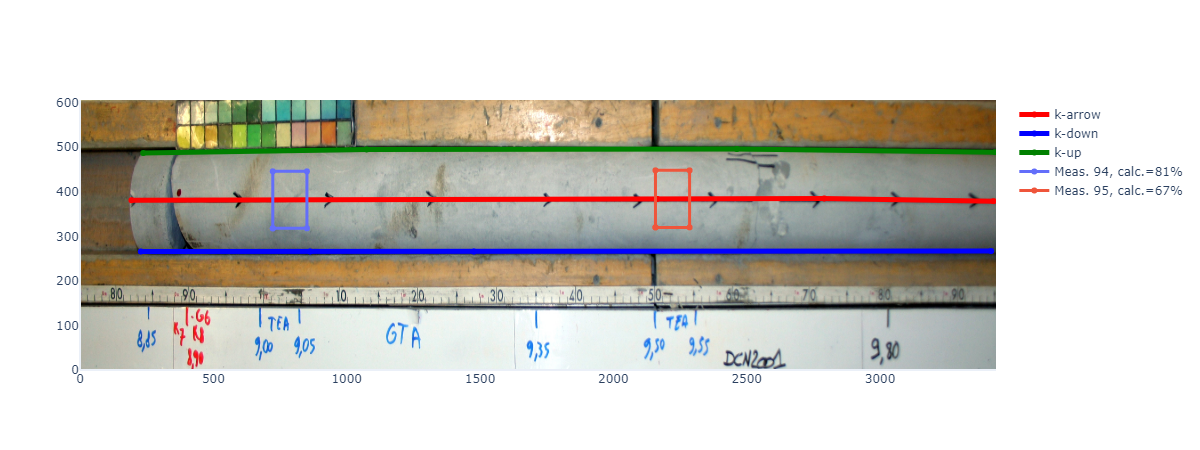
\includegraphics{./regression_files/drill_bpe4023.png}
\caption{core}
\end{figure}

The question is the following \textbf{regression} question:
\textgreater{} Is it possible to find a predictor able to estimate the
calcimetry value \(m_i\) only looking at the thumbnail image

\[
m_i = f(T)
\] where f is the regression function to be estimated.

\hypertarget{our-first-dataset}{%
\subsection{Our first dataset}\label{our-first-dataset}}

With a thumbnail of size 128, we got \textbf{4067} valid measurement
points that should be used. This defines the size of our dataset. Each
entry in the dataset is a tuple \((V_i, m_i)\)

    \begin{tcolorbox}[breakable, size=fbox, boxrule=1pt, pad at break*=1mm,colback=cellbackground, colframe=cellborder]
\prompt{In}{incolor}{1}{\boxspacing}
\begin{Verbatim}[commandchars=\\\{\}]
\PY{k+kn}{from} \PY{n+nn}{calcimetry}\PY{n+nn}{.}\PY{n+nn}{mongo\PYZus{}api} \PY{k+kn}{import} \PY{n}{MongoInfo}
\PY{k+kn}{from} \PY{n+nn}{calcimetry}\PY{n+nn}{.}\PY{n+nn}{thumbnail\PYZus{}api} \PY{k+kn}{import} \PY{n}{ThumbnailAPI}
\PY{k+kn}{from} \PY{n+nn}{PIL} \PY{k+kn}{import} \PY{n}{Image}
\PY{k+kn}{import} \PY{n+nn}{matplotlib}\PY{n+nn}{.}\PY{n+nn}{pyplot} \PY{k}{as} \PY{n+nn}{plt}
\PY{k+kn}{import} \PY{n+nn}{io}
\PY{k+kn}{import} \PY{n+nn}{random}
\PY{k+kn}{import} \PY{n+nn}{base64}

\PY{n}{HOST} \PY{o}{=} \PY{l+s+s1}{\PYZsq{}}\PY{l+s+s1}{localhost}\PY{l+s+s1}{\PYZsq{}}
\PY{n}{PORT} \PY{o}{=} \PY{l+m+mi}{27010}

\PY{c+c1}{\PYZsh{} Load Dataset}

\PY{n}{random}\PY{o}{.}\PY{n}{seed}\PY{p}{(}\PY{l+m+mi}{1}\PY{p}{)}

\PY{n}{mongo\PYZus{}info} \PY{o}{=} \PY{n}{MongoInfo}\PY{p}{(}\PY{n}{host}\PY{o}{=}\PY{n}{HOST}\PY{p}{,} \PY{n}{port}\PY{o}{=}\PY{n}{PORT}\PY{p}{)}
\PY{n}{thumb\PYZus{}list} \PY{o}{=} \PY{p}{[}\PY{p}{]}
\PY{k}{with} \PY{n}{ThumbnailAPI}\PY{p}{(}\PY{n}{mongo\PYZus{}info}\PY{o}{=}\PY{n}{mongo\PYZus{}info}\PY{p}{)} \PY{k}{as} \PY{n}{thumb\PYZus{}api}\PY{p}{:}
    \PY{n}{size} \PY{o}{=} \PY{n}{thumb\PYZus{}api}\PY{o}{.}\PY{n}{size}\PY{p}{(}\PY{p}{)}
    \PY{n+nb}{print}\PY{p}{(}\PY{n}{size}\PY{p}{)}
    \PY{k}{for} \PY{n}{i} \PY{o+ow}{in} \PY{n+nb}{range}\PY{p}{(}\PY{l+m+mi}{10}\PY{p}{)}\PY{p}{:}
        \PY{n}{idx} \PY{o}{=} \PY{n+nb}{int}\PY{p}{(}\PY{n}{random}\PY{o}{.}\PY{n}{random}\PY{p}{(}\PY{p}{)}\PY{o}{*}\PY{n}{size}\PY{p}{)}
        \PY{n}{thumb} \PY{o}{=} \PY{n}{thumb\PYZus{}api}\PY{o}{.}\PY{n}{read}\PY{p}{(}\PY{n}{idx}\PY{p}{)}
        \PY{n}{thumb\PYZus{}list}\PY{o}{.}\PY{n}{append}\PY{p}{(}\PY{n}{thumb}\PY{p}{)}
    \PY{c+c1}{\PYZsh{}plt.imshow(thumb)}
    
\end{Verbatim}
\end{tcolorbox}

    \begin{Verbatim}[commandchars=\\\{\}]
4067
    \end{Verbatim}

    As illustration, we draw above a collection of 10 samples randomly
selected among the 4067. In addition to the picture of the thumbnail
itself, an histogram of pixel values, the calcimetry measure at 1 minute
and the id of the core are also given. * To compute the histogram, each
RGB thumbnail image was first converted to a gray level image. * As each
core photo differs in resolution, the thumbnail picture was resized when
extracted so that the absolute size of the 128x128 pixels is the same
for all thumbnails.

    \begin{tcolorbox}[breakable, size=fbox, boxrule=1pt, pad at break*=1mm,colback=cellbackground, colframe=cellborder]
\prompt{In}{incolor}{2}{\boxspacing}
\begin{Verbatim}[commandchars=\\\{\}]
\PY{k+kn}{from} \PY{n+nn}{IPython}\PY{n+nn}{.}\PY{n+nn}{display} \PY{k+kn}{import} \PY{n}{Image}\PY{p}{,} \PY{n}{HTML}\PY{p}{,} \PY{n}{display}


\PY{k}{def} \PY{n+nf}{get\PYZus{}histo}\PY{p}{(}\PY{n}{img}\PY{p}{)}\PY{p}{:}
    \PY{n}{gray} \PY{o}{=} \PY{n}{img}\PY{o}{.}\PY{n}{convert}\PY{p}{(}\PY{l+s+s1}{\PYZsq{}}\PY{l+s+s1}{L}\PY{l+s+s1}{\PYZsq{}}\PY{p}{)}
    \PY{n}{fig}\PY{p}{,} \PY{n}{ax} \PY{o}{=} \PY{n}{plt}\PY{o}{.}\PY{n}{subplots}\PY{p}{(}\PY{n}{nrows}\PY{o}{=}\PY{l+m+mi}{1}\PY{p}{,} \PY{n}{ncols}\PY{o}{=}\PY{l+m+mi}{1}\PY{p}{)}
    \PY{n}{ax}\PY{o}{.}\PY{n}{set\PYZus{}axis\PYZus{}off}\PY{p}{(}\PY{p}{)}
    \PY{n}{ax}\PY{o}{.}\PY{n}{plot}\PY{p}{(}\PY{n}{gray}\PY{o}{.}\PY{n}{histogram}\PY{p}{(}\PY{p}{)}\PY{p}{)}
    \PY{n}{img\PYZus{}byte\PYZus{}array} \PY{o}{=} \PY{n}{io}\PY{o}{.}\PY{n}{BytesIO}\PY{p}{(}\PY{p}{)}
    \PY{n}{fig}\PY{o}{.}\PY{n}{savefig}\PY{p}{(}\PY{n}{img\PYZus{}byte\PYZus{}array}\PY{p}{,} \PY{n+nb}{format}\PY{o}{=}\PY{l+s+s1}{\PYZsq{}}\PY{l+s+s1}{jpeg}\PY{l+s+s1}{\PYZsq{}}\PY{p}{)}
    \PY{n}{plt}\PY{o}{.}\PY{n}{close}\PY{p}{(}\PY{n}{fig}\PY{p}{)}
    \PY{k}{return} \PY{n}{base64}\PY{o}{.}\PY{n}{b64encode}\PY{p}{(}\PY{n}{img\PYZus{}byte\PYZus{}array}\PY{o}{.}\PY{n}{getvalue}\PY{p}{(}\PY{p}{)}\PY{p}{)}\PY{o}{.}\PY{n}{decode}\PY{p}{(}\PY{p}{)}

\PY{k}{def} \PY{n+nf}{save\PYZus{}histo}\PY{p}{(}\PY{n}{img}\PY{p}{,} \PY{n}{filename}\PY{p}{)}\PY{p}{:}
    \PY{n}{gray} \PY{o}{=} \PY{n}{img}\PY{o}{.}\PY{n}{convert}\PY{p}{(}\PY{l+s+s1}{\PYZsq{}}\PY{l+s+s1}{L}\PY{l+s+s1}{\PYZsq{}}\PY{p}{)}

    \PY{n}{fig}\PY{p}{,} \PY{n}{ax} \PY{o}{=} \PY{n}{plt}\PY{o}{.}\PY{n}{subplots}\PY{p}{(}\PY{n}{nrows}\PY{o}{=}\PY{l+m+mi}{1}\PY{p}{,} \PY{n}{ncols}\PY{o}{=}\PY{l+m+mi}{1}\PY{p}{)}
    \PY{n}{ax}\PY{o}{.}\PY{n}{set\PYZus{}axis\PYZus{}off}\PY{p}{(}\PY{p}{)}
    \PY{n}{ax}\PY{o}{.}\PY{n}{plot}\PY{p}{(}\PY{n}{gray}\PY{o}{.}\PY{n}{histogram}\PY{p}{(}\PY{p}{)}\PY{p}{)}
    \PY{n}{fig}\PY{o}{.}\PY{n}{savefig}\PY{p}{(}\PY{n}{filename}\PY{p}{,} \PY{n+nb}{format}\PY{o}{=}\PY{l+s+s1}{\PYZsq{}}\PY{l+s+s1}{jpeg}\PY{l+s+s1}{\PYZsq{}}\PY{p}{)}
    \PY{n}{plt}\PY{o}{.}\PY{n}{close}\PY{p}{(}\PY{n}{fig}\PY{p}{)}


\PY{k}{def} \PY{n+nf}{to\PYZus{}base64}\PY{p}{(}\PY{n}{img}\PY{p}{:} \PY{n}{Image}\PY{p}{)}\PY{p}{:}
    \PY{n}{byte\PYZus{}array} \PY{o}{=} \PY{n}{io}\PY{o}{.}\PY{n}{BytesIO}\PY{p}{(}\PY{p}{)}
    \PY{n}{img}\PY{o}{.}\PY{n}{save}\PY{p}{(}\PY{n}{byte\PYZus{}array}\PY{p}{,} \PY{n+nb}{format}\PY{o}{=}\PY{l+s+s1}{\PYZsq{}}\PY{l+s+s1}{jpeg}\PY{l+s+s1}{\PYZsq{}}\PY{p}{)}
    \PY{k}{return} \PY{n}{base64}\PY{o}{.}\PY{n}{b64encode}\PY{p}{(}\PY{n}{byte\PYZus{}array}\PY{o}{.}\PY{n}{getvalue}\PY{p}{(}\PY{p}{)}\PY{p}{)}\PY{o}{.}\PY{n}{decode}\PY{p}{(}\PY{p}{)}


\PY{n}{html\PYZus{}str} \PY{o}{=} \PY{l+s+s2}{\PYZdq{}}\PY{l+s+s2}{\PYZlt{}div style=}\PY{l+s+s2}{\PYZsq{}}\PY{l+s+s2}{display: inline\PYZhy{}block; align:justify; border: 1px solid white;}\PY{l+s+s2}{\PYZsq{}}\PY{l+s+s2}{\PYZgt{}}\PY{l+s+s2}{\PYZdq{}}
\PY{n}{html\PYZus{}str} \PY{o}{+}\PY{o}{=}\PY{l+s+s2}{\PYZdq{}}\PY{l+s+s2}{\PYZlt{}img style=}\PY{l+s+s2}{\PYZsq{}}\PY{l+s+s2}{width: 128px; margin: 0px; float: left; }\PY{l+s+s2}{\PYZsq{}}\PY{l+s+s2}{src=}\PY{l+s+s2}{\PYZsq{}}\PY{l+s+s2}{./regression\PYZus{}files/images\PYZus{}}\PY{l+s+si}{\PYZpc{}d}\PY{l+s+s2}{.jpg}\PY{l+s+s2}{\PYZsq{}}\PY{l+s+s2}{ /\PYZgt{}}\PY{l+s+s2}{\PYZdq{}}
\PY{n}{html\PYZus{}str} \PY{o}{+}\PY{o}{=} \PY{l+s+s2}{\PYZdq{}}\PY{l+s+s2}{\PYZlt{}img style=}\PY{l+s+s2}{\PYZsq{}}\PY{l+s+s2}{width: 128px; margin: 0px; float: left; }\PY{l+s+s2}{\PYZsq{}}\PY{l+s+s2}{ src=}\PY{l+s+s2}{\PYZsq{}}\PY{l+s+s2}{./regression\PYZus{}files/histo\PYZus{}}\PY{l+s+si}{\PYZpc{}d}\PY{l+s+s2}{.jpg}\PY{l+s+s2}{\PYZsq{}}\PY{l+s+s2}{ /\PYZgt{}}\PY{l+s+s2}{\PYZdq{}}
\PY{n}{html\PYZus{}str} \PY{o}{+}\PY{o}{=}\PY{l+s+s2}{\PYZdq{}}\PY{l+s+s2}{\PYZlt{}P style=}\PY{l+s+s2}{\PYZsq{}}\PY{l+s+s2}{text\PYZhy{}align: center;}\PY{l+s+s2}{\PYZsq{}}\PY{l+s+s2}{\PYZgt{}}\PY{l+s+si}{\PYZpc{}s}\PY{l+s+s2}{ (}\PY{l+s+si}{\PYZpc{}s}\PY{l+s+s2}{)\PYZlt{}/P\PYZgt{}}\PY{l+s+s2}{\PYZdq{}}
\PY{n}{html\PYZus{}str} \PY{o}{+}\PY{o}{=}\PY{l+s+s2}{\PYZdq{}}\PY{l+s+s2}{\PYZlt{}/div\PYZgt{}}\PY{l+s+se}{\PYZbs{}n}\PY{l+s+s2}{\PYZdq{}}


\PY{n}{all\PYZus{}str} \PY{o}{=} \PY{l+s+s2}{\PYZdq{}}\PY{l+s+s2}{ }\PY{l+s+s2}{\PYZdq{}}
\PY{k}{for} \PY{n}{i}\PY{p}{,} \PY{n}{t} \PY{o+ow}{in} \PY{n+nb}{enumerate}\PY{p}{(}\PY{n}{thumb\PYZus{}list}\PY{p}{)}\PY{p}{:}
    \PY{n}{t}\PY{o}{.}\PY{n}{jpg}\PY{o}{.}\PY{n}{save}\PY{p}{(}\PY{l+s+sa}{f}\PY{l+s+s2}{\PYZdq{}}\PY{l+s+s2}{./regression\PYZus{}files/images\PYZus{}}\PY{l+s+si}{\PYZob{}}\PY{n}{i}\PY{l+s+si}{\PYZcb{}}\PY{l+s+s2}{.jpg}\PY{l+s+s2}{\PYZdq{}}\PY{p}{,} \PY{n+nb}{format}\PY{o}{=}\PY{l+s+s2}{\PYZdq{}}\PY{l+s+s2}{jpeg}\PY{l+s+s2}{\PYZdq{}}\PY{p}{)}
    \PY{n}{save\PYZus{}histo}\PY{p}{(}\PY{n}{t}\PY{o}{.}\PY{n}{jpg}\PY{p}{,} \PY{l+s+sa}{f}\PY{l+s+s2}{\PYZdq{}}\PY{l+s+s2}{./regression\PYZus{}files/histo\PYZus{}}\PY{l+s+si}{\PYZob{}}\PY{n}{i}\PY{l+s+si}{\PYZcb{}}\PY{l+s+s2}{.jpg}\PY{l+s+s2}{\PYZdq{}}\PY{p}{)}
    \PY{n}{all\PYZus{}str} \PY{o}{+}\PY{o}{=} \PY{n}{html\PYZus{}str} \PY{o}{\PYZpc{}} \PY{p}{(}\PY{n}{i}\PY{p}{,} \PY{n}{i}\PY{p}{,} \PY{n}{t}\PY{o}{.}\PY{n}{measurement}\PY{o}{.}\PY{n}{val\PYZus{}1m}\PY{p}{,} \PY{n}{t}\PY{o}{.}\PY{n}{measurement}\PY{o}{.}\PY{n}{image\PYZus{}id}\PY{p}{)}
\PY{n}{HTML}\PY{p}{(}\PY{n}{all\PYZus{}str}\PY{p}{)}
\end{Verbatim}
\end{tcolorbox}

            \begin{tcolorbox}[breakable, size=fbox, boxrule=.5pt, pad at break*=1mm, opacityfill=0]
\prompt{Out}{outcolor}{2}{\boxspacing}
\begin{Verbatim}[commandchars=\\\{\}]
<IPython.core.display.HTML object>
\end{Verbatim}
\end{tcolorbox}
        
    \hypertarget{features}{%
\subsection{Features}\label{features}}

To begin instead of predicting the calcimetry using directly the
thumbnail pixel's matrix, a ``feature'' approach was tried. On each
thumbnail, some features are then computed * \texttt{Focus} : The
variance of the Laplacian can be a measure of the sharpness of the
image, or the focus. * \texttt{Gradient} : Magnitude of the gradient to
get sharpness of edges, calculate maximum and standard deviation. *
\texttt{Colours} : The top five colours in the image from clustering
analysis * \texttt{BRISQUE} : blind/referenceless image spatial quality
evaluator

See for further information -
\href{https://towardsdatascience.com/building-an-image-color-analyzer-using-python-12de6b0acf74}{Colour
Analysis} -
\href{https://github.com/photosynthesis-team/piq/blob/master/examples/image_metrics.py}{Pytorch
Image Quality} - \href{../notebooks/image-quality-talk.ipynb}{Image
Quality Notebook}

As it was guess that somehow calcimetry was related with some grey
level, some other features are also defined. * \texttt{mean\_color} that
is the mean of all \texttt{Colours} previously defined. *
\texttt{bin-1..5} that are 5 features build computing one 5 bins
histogram on each thumbnail

The following table summarizes all the features used in a first step
once converted to pandas dataframe. To complete the dataset, the last
column gives the expected calcimetry value expected to be deduced from
this features.

    \begin{tcolorbox}[breakable, size=fbox, boxrule=1pt, pad at break*=1mm,colback=cellbackground, colframe=cellborder]
\prompt{In}{incolor}{3}{\boxspacing}
\begin{Verbatim}[commandchars=\\\{\}]
\PY{k+kn}{import} \PY{n+nn}{pandas} \PY{k}{as} \PY{n+nn}{pd}
\PY{k+kn}{import} \PY{n+nn}{numpy} \PY{k}{as} \PY{n+nn}{np}
\PY{k+kn}{from} \PY{n+nn}{calcimetry}\PY{n+nn}{.}\PY{n+nn}{thumbnail\PYZus{}api} \PY{k+kn}{import} \PY{n}{ThumbnailAPI}

\PY{n}{n\PYZus{}bins} \PY{o}{=} \PY{l+m+mi}{6}
\PY{k}{def} \PY{n+nf}{get\PYZus{}histo}\PY{p}{(}\PY{n}{t}\PY{p}{,} \PY{n}{n\PYZus{}bins}\PY{p}{)}\PY{p}{:}
    \PY{n}{w}\PY{p}{,} \PY{n}{h} \PY{o}{=} \PY{n}{t}\PY{o}{.}\PY{n}{jpg}\PY{o}{.}\PY{n}{size}
    \PY{n}{histo}\PY{p}{,} \PY{n}{bins} \PY{o}{=} \PY{n}{np}\PY{o}{.}\PY{n}{histogram}\PY{p}{(}\PY{n}{t}\PY{o}{.}\PY{n}{jpg}\PY{p}{,} \PY{n}{bins}\PY{o}{=}\PY{n}{n\PYZus{}bins}\PY{p}{)}
    \PY{k}{return} \PY{n}{histo}\PY{o}{.}\PY{n}{astype}\PY{p}{(}\PY{n}{np}\PY{o}{.}\PY{n}{float64}\PY{p}{)} \PY{o}{/} \PY{p}{(}\PY{n}{w}\PY{o}{*}\PY{n}{h}\PY{p}{)}

\PY{c+c1}{\PYZsh{}create dataframe for learing}
\PY{n}{columns} \PY{o}{=} \PY{p}{[}
    \PY{l+s+s2}{\PYZdq{}}\PY{l+s+s2}{focus}\PY{l+s+s2}{\PYZdq{}}\PY{p}{,} \PY{l+s+s2}{\PYZdq{}}\PY{l+s+s2}{mean\PYZus{}grad}\PY{l+s+s2}{\PYZdq{}}\PY{p}{,} \PY{l+s+s2}{\PYZdq{}}\PY{l+s+s2}{mean\PYZus{}color}\PY{l+s+s2}{\PYZdq{}}\PY{p}{,} \PY{l+s+s2}{\PYZdq{}}\PY{l+s+s2}{brisque}\PY{l+s+s2}{\PYZdq{}}
\PY{p}{]}
\PY{k}{for} \PY{n}{i} \PY{o+ow}{in} \PY{n+nb}{range}\PY{p}{(}\PY{n}{n\PYZus{}bins}\PY{p}{)}\PY{p}{:}
    \PY{n}{columns}\PY{o}{.}\PY{n}{append}\PY{p}{(}\PY{l+s+sa}{f}\PY{l+s+s2}{\PYZdq{}}\PY{l+s+s2}{bin\PYZus{}}\PY{l+s+si}{\PYZob{}}\PY{n}{i}\PY{l+s+si}{\PYZcb{}}\PY{l+s+s2}{\PYZdq{}}\PY{p}{)}
\PY{n}{columns}\PY{o}{.}\PY{n}{append}\PY{p}{(}\PY{l+s+s1}{\PYZsq{}}\PY{l+s+s1}{target}\PY{l+s+s1}{\PYZsq{}}\PY{p}{)}
    
\PY{n}{data} \PY{o}{=} \PY{p}{[}\PY{p}{]}

\PY{k}{with} \PY{n}{ThumbnailAPI}\PY{p}{(}\PY{n}{mongo\PYZus{}info}\PY{o}{=}\PY{n}{mongo\PYZus{}info}\PY{p}{)} \PY{k}{as} \PY{n}{thumb\PYZus{}api}\PY{p}{:}
    \PY{n}{size} \PY{o}{=} \PY{n}{thumb\PYZus{}api}\PY{o}{.}\PY{n}{size}\PY{p}{(}\PY{p}{)}    
    \PY{k}{for} \PY{n}{idx} \PY{o+ow}{in} \PY{n+nb}{range}\PY{p}{(}\PY{n}{size}\PY{p}{)}\PY{p}{:}
        \PY{c+c1}{\PYZsh{}idx = int(random.random()*size)}
        \PY{n}{t} \PY{o}{=} \PY{n}{thumb\PYZus{}api}\PY{o}{.}\PY{n}{read}\PY{p}{(}\PY{n}{idx}\PY{p}{)}
        \PY{n}{row} \PY{o}{=} \PY{p}{[}\PY{n}{t}\PY{o}{.}\PY{n}{quality}\PY{o}{.}\PY{n}{focus}\PY{p}{,} \PY{n}{t}\PY{o}{.}\PY{n}{quality}\PY{o}{.}\PY{n}{gradient}\PY{p}{[}\PY{l+s+s1}{\PYZsq{}}\PY{l+s+s1}{ave}\PY{l+s+s1}{\PYZsq{}}\PY{p}{]}\PY{p}{,} \PY{n}{np}\PY{o}{.}\PY{n}{mean}\PY{p}{(}\PY{n}{t}\PY{o}{.}\PY{n}{quality}\PY{o}{.}\PY{n}{colours}\PY{p}{)}\PY{p}{,} \PY{n}{t}\PY{o}{.}\PY{n}{quality}\PY{o}{.}\PY{n}{brisque}\PY{p}{]}
        \PY{n}{histo} \PY{o}{=} \PY{n}{get\PYZus{}histo}\PY{p}{(}\PY{n}{t}\PY{p}{,} \PY{n}{n\PYZus{}bins}\PY{p}{)}
        \PY{k}{for} \PY{n}{i} \PY{o+ow}{in} \PY{n+nb}{range}\PY{p}{(}\PY{n}{n\PYZus{}bins}\PY{p}{)}\PY{p}{:}
            \PY{n}{row}\PY{o}{.}\PY{n}{append}\PY{p}{(}\PY{n}{histo}\PY{p}{[}\PY{n}{i}\PY{p}{]}\PY{p}{)}
        \PY{n}{row}\PY{o}{.}\PY{n}{append}\PY{p}{(}\PY{n+nb}{float}\PY{p}{(}\PY{n}{t}\PY{o}{.}\PY{n}{measurement}\PY{o}{.}\PY{n}{val\PYZus{}1m}\PY{p}{)}\PY{p}{)}
        \PY{n}{data}\PY{o}{.}\PY{n}{append}\PY{p}{(}\PY{n}{row}\PY{p}{)}
    
\PY{n}{df} \PY{o}{=} \PY{n}{pd}\PY{o}{.}\PY{n}{DataFrame}\PY{p}{(}\PY{n}{data}\PY{p}{,} \PY{n}{columns}\PY{o}{=}\PY{n}{columns}\PY{p}{)}
\PY{n}{df}\PY{o}{.}\PY{n}{head}\PY{p}{(}\PY{p}{)}
\end{Verbatim}
\end{tcolorbox}

            \begin{tcolorbox}[breakable, size=fbox, boxrule=.5pt, pad at break*=1mm, opacityfill=0]
\prompt{Out}{outcolor}{3}{\boxspacing}
\begin{Verbatim}[commandchars=\\\{\}]
        focus  mean\_grad  mean\_color    brisque     bin\_0     bin\_1     bin\_2  \textbackslash{}
0  168.300274  42.614488   93.551401  25.967468  0.008850  0.133545  0.891785
1  118.353516  32.405043   89.971384  20.834656  0.032227  0.120605  0.831970
2  110.426135  32.370667   85.950415  26.956238  0.040649  0.094604  0.588196
3   97.795724  29.870769   77.753587  28.365417  0.039551  0.114563  0.664185
4   87.493495  28.363839   68.290218  23.031433  0.050659  0.149353  0.711792

      bin\_3     bin\_4     bin\_5  target
0  1.164612  0.733643  0.067566    29.0
1  1.268433  0.739990  0.006775    31.0
2  0.704224  1.201477  0.370850    33.0
3  0.872192  1.042480  0.267029    33.0
4  0.901733  0.977112  0.209351    33.0
\end{Verbatim}
\end{tcolorbox}
        
    \hypertarget{normalization}{%
\subsubsection{Normalization}\label{normalization}}

    As our features don't use the same range, a \(z_i=(x_i-\mu_i)/\sigma_i\)
normalization is performed to scale each feature in \([0,1]\) range

    \begin{tcolorbox}[breakable, size=fbox, boxrule=1pt, pad at break*=1mm,colback=cellbackground, colframe=cellborder]
\prompt{In}{incolor}{4}{\boxspacing}
\begin{Verbatim}[commandchars=\\\{\}]
\PY{n}{normalized\PYZus{}df} \PY{o}{=} \PY{n}{df}\PY{o}{.}\PY{n}{copy}\PY{p}{(}\PY{p}{)}
\PY{k}{for} \PY{n}{c} \PY{o+ow}{in} \PY{n}{columns}\PY{p}{:}
    \PY{k}{if} \PY{n}{c} \PY{o}{==} \PY{l+s+s1}{\PYZsq{}}\PY{l+s+s1}{target}\PY{l+s+s1}{\PYZsq{}}\PY{p}{:}
        \PY{k}{continue}
    \PY{n}{mean} \PY{o}{=} \PY{n}{normalized\PYZus{}df}\PY{p}{[}\PY{n}{c}\PY{p}{]}\PY{o}{.}\PY{n}{mean}\PY{p}{(}\PY{p}{)}
    \PY{n}{std} \PY{o}{=} \PY{n}{normalized\PYZus{}df}\PY{p}{[}\PY{n}{c}\PY{p}{]}\PY{o}{.}\PY{n}{std}\PY{p}{(}\PY{p}{)}
    \PY{n}{normalized\PYZus{}df}\PY{p}{[}\PY{n}{c}\PY{p}{]} \PY{o}{=} \PY{p}{(}\PY{n}{df}\PY{p}{[}\PY{n}{c}\PY{p}{]} \PY{o}{\PYZhy{}} \PY{n}{mean}\PY{p}{)} \PY{o}{/} \PY{n}{std} 

\PY{n}{normalized\PYZus{}df}\PY{o}{.}\PY{n}{head}\PY{p}{(}\PY{p}{)}
\end{Verbatim}
\end{tcolorbox}

            \begin{tcolorbox}[breakable, size=fbox, boxrule=.5pt, pad at break*=1mm, opacityfill=0]
\prompt{Out}{outcolor}{4}{\boxspacing}
\begin{Verbatim}[commandchars=\\\{\}]
      focus  mean\_grad  mean\_color   brisque     bin\_0     bin\_1     bin\_2  \textbackslash{}
0 -0.048182   0.471487   -0.397528 -0.197146 -0.604047 -0.294992  0.929507
1 -0.300642  -0.388002   -0.519708 -0.613800 -0.394549 -0.344614  0.797319
2 -0.340712  -0.390896   -0.656938 -0.116883 -0.319064 -0.444328  0.258585
3 -0.404553  -0.601352   -0.936684 -0.002494 -0.328910 -0.367787  0.426518
4 -0.456627  -0.728214   -1.259654 -0.435478 -0.229357 -0.234368  0.531729

      bin\_3     bin\_4     bin\_5  target
0  0.557339 -0.514068 -0.576702    29.0
1  0.763671 -0.504145 -0.730560    31.0
2 -0.357629  0.217261  0.190889    33.0
3 -0.023810 -0.031286 -0.071875    33.0
4  0.034899 -0.133472 -0.217854    33.0
\end{Verbatim}
\end{tcolorbox}
        
    \hypertarget{exploring-the-dataset}{%
\subsection{Exploring the dataset}\label{exploring-the-dataset}}

Visual exploration of the dataset is always a good way to discover
information contained in data A correlation pairplot is then displayed
to have a better look which characteristics are correlated with each
others.

    \begin{tcolorbox}[breakable, size=fbox, boxrule=1pt, pad at break*=1mm,colback=cellbackground, colframe=cellborder]
\prompt{In}{incolor}{5}{\boxspacing}
\begin{Verbatim}[commandchars=\\\{\}]
\PY{k+kn}{import} \PY{n+nn}{seaborn} \PY{k}{as} \PY{n+nn}{sns}

\PY{c+c1}{\PYZsh{} Here are selected some features to be plot.}
\PY{n}{selected\PYZus{}df} \PY{o}{=} \PY{n}{normalized\PYZus{}df}\PY{p}{[}\PY{p}{[}\PY{l+s+s1}{\PYZsq{}}\PY{l+s+s1}{focus}\PY{l+s+s1}{\PYZsq{}}\PY{p}{,} \PY{l+s+s1}{\PYZsq{}}\PY{l+s+s1}{mean\PYZus{}grad}\PY{l+s+s1}{\PYZsq{}}\PY{p}{,} \PY{l+s+s2}{\PYZdq{}}\PY{l+s+s2}{brisque}\PY{l+s+s2}{\PYZdq{}}\PY{p}{,} \PY{l+s+s2}{\PYZdq{}}\PY{l+s+s2}{bin\PYZus{}3}\PY{l+s+s2}{\PYZdq{}}\PY{p}{]}\PY{p}{]}
\PY{n}{sns}\PY{o}{.}\PY{n}{pairplot}\PY{p}{(}\PY{n}{selected\PYZus{}df}\PY{p}{)}
\end{Verbatim}
\end{tcolorbox}

            \begin{tcolorbox}[breakable, size=fbox, boxrule=.5pt, pad at break*=1mm, opacityfill=0]
\prompt{Out}{outcolor}{5}{\boxspacing}
\begin{Verbatim}[commandchars=\\\{\}]
<seaborn.axisgrid.PairGrid at 0x196c95f3c10>
\end{Verbatim}
\end{tcolorbox}
        
    \begin{center}
    \adjustimage{max size={0.9\linewidth}{0.9\paperheight}}{regression_files/regression_10_1.png}
    \end{center}
    { \hspace*{\fill} \\}
    
    Then a correlation matrix can also be computed.

    \begin{tcolorbox}[breakable, size=fbox, boxrule=1pt, pad at break*=1mm,colback=cellbackground, colframe=cellborder]
\prompt{In}{incolor}{6}{\boxspacing}
\begin{Verbatim}[commandchars=\\\{\}]
\PY{k+kn}{import} \PY{n+nn}{seaborn} \PY{k}{as} \PY{n+nn}{sns} \PY{c+c1}{\PYZsh{}visualization package}
\PY{n}{corr} \PY{o}{=} \PY{n}{normalized\PYZus{}df}\PY{o}{.}\PY{n}{corr}\PY{p}{(}\PY{p}{)}
\PY{n}{plt}\PY{o}{.}\PY{n}{subplots}\PY{p}{(}\PY{n}{figsize}\PY{o}{=}\PY{p}{(}\PY{l+m+mi}{8}\PY{p}{,}\PY{l+m+mi}{8}\PY{p}{)}\PY{p}{)}
\PY{n}{sns}\PY{o}{.}\PY{n}{heatmap}\PY{p}{(}\PY{n}{corr}\PY{p}{,}\PY{n}{cmap}\PY{o}{=} \PY{l+s+s1}{\PYZsq{}}\PY{l+s+s1}{RdYlGn}\PY{l+s+s1}{\PYZsq{}}\PY{p}{,}\PY{n}{annot}\PY{o}{=}\PY{k+kc}{True}\PY{p}{)}
\PY{n}{plt}\PY{o}{.}\PY{n}{show}\PY{p}{(}\PY{p}{)}
\end{Verbatim}
\end{tcolorbox}

    \begin{center}
    \adjustimage{max size={0.9\linewidth}{0.9\paperheight}}{regression_files/regression_12_0.png}
    \end{center}
    { \hspace*{\fill} \\}
    
    \begin{itemize}
\tightlist
\item
  As it can be seen on \texttt{pairplot} some features are highly
  correlated as \texttt{focus} with \texttt{mean\_grad}
\item
  In this matrix, it can be seen that the \texttt{target} (calcimetry)
  is poorly correlated with each feature if invidualy considered.
\end{itemize}

    \hypertarget{histogram-of-calcimetry-values.}{%
\subsubsection{Histogram of calcimetry
values.}\label{histogram-of-calcimetry-values.}}

The histogram of all calcimetry values shows clearly that values in
range \([15, 35]\) are clearly overrepresented. This may lead to a
regression model that is not equaly accurate on the whole range and
mostly for high calcimetry values

    \begin{tcolorbox}[breakable, size=fbox, boxrule=1pt, pad at break*=1mm,colback=cellbackground, colframe=cellborder]
\prompt{In}{incolor}{9}{\boxspacing}
\begin{Verbatim}[commandchars=\\\{\}]
\PY{n}{hist}\PY{o}{=}  \PY{n}{plt}\PY{o}{.}\PY{n}{hist}\PY{p}{(}\PY{n}{df}\PY{p}{[}\PY{l+s+s1}{\PYZsq{}}\PY{l+s+s1}{target}\PY{l+s+s1}{\PYZsq{}}\PY{p}{]}\PY{p}{)}
\end{Verbatim}
\end{tcolorbox}

    \begin{center}
    \adjustimage{max size={0.9\linewidth}{0.9\paperheight}}{regression_files/regression_15_0.png}
    \end{center}
    { \hspace*{\fill} \\}
    
    \hypertarget{performing-regression}{%
\subsection{Performing regression}\label{performing-regression}}

\hypertarget{training}{%
\subsubsection{Training}\label{training}}

Remember performing regression is equivalent to find \(f\) (learning
parameters) so that \(y=f(x)\) where \(y\) is our calcimetry and \(x\)
is a vector built using all normalized features.

    \begin{tcolorbox}[breakable, size=fbox, boxrule=1pt, pad at break*=1mm,colback=cellbackground, colframe=cellborder]
\prompt{In}{incolor}{10}{\boxspacing}
\begin{Verbatim}[commandchars=\\\{\}]
\PY{c+c1}{\PYZsh{}independent variables / explanatory variables / features}
\PY{n}{x} \PY{o}{=} \PY{n}{normalized\PYZus{}df}\PY{o}{.}\PY{n}{drop}\PY{p}{(}\PY{n}{labels}\PY{o}{=}\PY{l+s+s1}{\PYZsq{}}\PY{l+s+s1}{target}\PY{l+s+s1}{\PYZsq{}}\PY{p}{,} \PY{n}{axis}\PY{o}{=}\PY{l+m+mi}{1}\PY{p}{)}  \PY{c+c1}{\PYZsh{}axis=1 means we drop data by column.}

\PY{c+c1}{\PYZsh{}dependent variable / response / target variable / calcimetry}
\PY{n}{y} \PY{o}{=} \PY{n}{normalized\PYZus{}df}\PY{p}{[}\PY{l+s+s1}{\PYZsq{}}\PY{l+s+s1}{target}\PY{l+s+s1}{\PYZsq{}}\PY{p}{]}
\end{Verbatim}
\end{tcolorbox}

    Our dataset need to be split in two : 1. A \textbf{training} dataset
that will be used to estimated paramaters of our models
(\textasciitilde80\% of the dataset) 1. A \textbf{testing} dataset that
will be kept to test who good is our model to predict calcimetry2) On
scinde en dataset d'apprentissage et de validation

    \begin{tcolorbox}[breakable, size=fbox, boxrule=1pt, pad at break*=1mm,colback=cellbackground, colframe=cellborder]
\prompt{In}{incolor}{11}{\boxspacing}
\begin{Verbatim}[commandchars=\\\{\}]
\PY{k+kn}{from} \PY{n+nn}{sklearn}\PY{n+nn}{.}\PY{n+nn}{model\PYZus{}selection} \PY{k+kn}{import} \PY{n}{train\PYZus{}test\PYZus{}split}
\PY{c+c1}{\PYZsh{}splitting the dataset into 80\PYZpc{}\PYZhy{}20\PYZpc{} train\PYZhy{}test split }
\PY{n}{train\PYZus{}x}\PY{p}{,} \PY{n}{test\PYZus{}x}\PY{p}{,} \PY{n}{train\PYZus{}y}\PY{p}{,} \PY{n}{test\PYZus{}y} \PY{o}{=} \PY{n}{train\PYZus{}test\PYZus{}split}\PY{p}{(}\PY{n}{x}\PY{p}{,}\PY{n}{y}\PY{p}{,}\PY{n}{test\PYZus{}size}\PY{o}{=}\PY{l+m+mf}{0.10}\PY{p}{,}\PY{n}{random\PYZus{}state}\PY{o}{=}\PY{l+m+mi}{123}\PY{p}{)}
\PY{n+nb}{print}\PY{p}{(}\PY{n}{train\PYZus{}x}\PY{o}{.}\PY{n}{shape}\PY{p}{)}
\PY{n+nb}{print}\PY{p}{(}\PY{n}{test\PYZus{}x}\PY{o}{.}\PY{n}{shape}\PY{p}{)}
\PY{n+nb}{print}\PY{p}{(}\PY{n}{train\PYZus{}y}\PY{o}{.}\PY{n}{shape}\PY{p}{)}
\PY{n+nb}{print}\PY{p}{(}\PY{n}{test\PYZus{}y}\PY{o}{.}\PY{n}{shape}\PY{p}{)}
\end{Verbatim}
\end{tcolorbox}

    \begin{Verbatim}[commandchars=\\\{\}]
(3660, 10)
(407, 10)
(3660,)
(407,)
    \end{Verbatim}

    Then regression is performed. Different models are available for
regression in the following cell from the simple one (\texttt{linear})
to more complicated (\texttt{extra\_tree}). In the following results are
given for the \emph{MultiLayerPerceptron}

    \begin{tcolorbox}[breakable, size=fbox, boxrule=1pt, pad at break*=1mm,colback=cellbackground, colframe=cellborder]
\prompt{In}{incolor}{12}{\boxspacing}
\begin{Verbatim}[commandchars=\\\{\}]
\PY{k+kn}{from} \PY{n+nn}{sklearn}\PY{n+nn}{.}\PY{n+nn}{linear\PYZus{}model} \PY{k+kn}{import} \PY{n}{BayesianRidge}\PY{p}{,} \PY{n}{LinearRegression}\PY{p}{,} \PY{n}{ARDRegression}
\PY{k+kn}{from} \PY{n+nn}{sklearn}\PY{n+nn}{.}\PY{n+nn}{neural\PYZus{}network} \PY{k+kn}{import} \PY{n}{MLPRegressor}
\PY{k+kn}{from} \PY{n+nn}{sklearn}\PY{n+nn}{.}\PY{n+nn}{ensemble} \PY{k+kn}{import} \PY{n}{ExtraTreesRegressor}     

\PY{k}{def} \PY{n+nf}{get\PYZus{}model}\PY{p}{(}\PY{n}{kind}\PY{p}{)}\PY{p}{:}
    \PY{k}{return} \PY{p}{\PYZob{}} 
        \PY{l+s+s1}{\PYZsq{}}\PY{l+s+s1}{ridge}\PY{l+s+s1}{\PYZsq{}}\PY{p}{:} \PY{n}{BayesianRidge}\PY{p}{(}\PY{p}{)}\PY{p}{,} 
        \PY{l+s+s1}{\PYZsq{}}\PY{l+s+s1}{linear}\PY{l+s+s1}{\PYZsq{}}\PY{p}{:} \PY{n}{LinearRegression}\PY{p}{(}\PY{p}{)}\PY{p}{,} 
        \PY{l+s+s2}{\PYZdq{}}\PY{l+s+s2}{ard}\PY{l+s+s2}{\PYZdq{}}\PY{p}{:} \PY{n}{ARDRegression}\PY{p}{(}\PY{p}{)}\PY{p}{,}
        \PY{l+s+s2}{\PYZdq{}}\PY{l+s+s2}{mlp}\PY{l+s+s2}{\PYZdq{}}\PY{p}{:} \PY{n}{MLPRegressor}\PY{p}{(}\PY{n}{max\PYZus{}iter}\PY{o}{=}\PY{l+m+mi}{1000}\PY{p}{,} \PY{n}{solver}\PY{o}{=}\PY{l+s+s1}{\PYZsq{}}\PY{l+s+s1}{sgd}\PY{l+s+s1}{\PYZsq{}}\PY{p}{,} \PY{n}{learning\PYZus{}rate}\PY{o}{=}\PY{l+s+s2}{\PYZdq{}}\PY{l+s+s2}{adaptive}\PY{l+s+s2}{\PYZdq{}}\PY{p}{)}\PY{p}{,}
        \PY{l+s+s2}{\PYZdq{}}\PY{l+s+s2}{extra\PYZus{}tree}\PY{l+s+s2}{\PYZdq{}}\PY{p}{:} \PY{n}{ExtraTreesRegressor}\PY{p}{(}\PY{n}{n\PYZus{}estimators}\PY{o}{=}\PY{l+m+mi}{100}\PY{p}{,} \PY{n}{random\PYZus{}state}\PY{o}{=}\PY{l+m+mi}{123}\PY{p}{)}
        \PY{p}{\PYZcb{}}\PY{p}{[}\PY{n}{kind}\PY{p}{]}
   

\PY{n}{lm} \PY{o}{=} \PY{n}{get\PYZus{}model}\PY{p}{(}\PY{l+s+s1}{\PYZsq{}}\PY{l+s+s1}{mlp}\PY{l+s+s1}{\PYZsq{}}\PY{p}{)}
\PY{n}{lm}\PY{o}{.}\PY{n}{fit}\PY{p}{(}\PY{n}{train\PYZus{}x}\PY{p}{,} \PY{n}{train\PYZus{}y}\PY{p}{)}
\end{Verbatim}
\end{tcolorbox}

            \begin{tcolorbox}[breakable, size=fbox, boxrule=.5pt, pad at break*=1mm, opacityfill=0]
\prompt{Out}{outcolor}{12}{\boxspacing}
\begin{Verbatim}[commandchars=\\\{\}]
MLPRegressor(learning\_rate='adaptive', max\_iter=1000, solver='sgd')
\end{Verbatim}
\end{tcolorbox}
        
    Selected model can then be used to estimate calcimetry from features on
train and test dataset and r2, q2 scores can then be computed. An
evaluation metric for regression issues is the R squared score, which
represents the percentage of variance in the target variable that is
explained by the model. R squared is a performance metric with a range
of 0 to 1, with larger values signifying better results. A model that
performs worse than one that merely predicts the mean value of the
target variable has a negative R squared value. In this instance, the
model is most certainly overfitting the data as indicated by the
negative R squared. A model learns to fit the noise in the data rather
than the underlying pattern when it overfits, which leads to poor
generalization to fresh data.

    \begin{tcolorbox}[breakable, size=fbox, boxrule=1pt, pad at break*=1mm,colback=cellbackground, colframe=cellborder]
\prompt{In}{incolor}{13}{\boxspacing}
\begin{Verbatim}[commandchars=\\\{\}]
\PY{n}{y\PYZus{}test\PYZus{}predicted} \PY{o}{=} \PY{n}{lm}\PY{o}{.}\PY{n}{predict}\PY{p}{(}\PY{n}{test\PYZus{}x}\PY{p}{)}
\PY{n}{y\PYZus{}train\PYZus{}predicted} \PY{o}{=} \PY{n}{lm}\PY{o}{.}\PY{n}{predict}\PY{p}{(}\PY{n}{train\PYZus{}x}\PY{p}{)}
\end{Verbatim}
\end{tcolorbox}

    \begin{tcolorbox}[breakable, size=fbox, boxrule=1pt, pad at break*=1mm,colback=cellbackground, colframe=cellborder]
\prompt{In}{incolor}{12}{\boxspacing}
\begin{Verbatim}[commandchars=\\\{\}]
\PY{k+kn}{from} \PY{n+nn}{sklearn} \PY{k+kn}{import} \PY{n}{metrics} \PY{k}{as} \PY{n}{mt}
\PY{n+nb}{print}\PY{p}{(}\PY{l+s+s2}{\PYZdq{}}\PY{l+s+s2}{1) The model explains,}\PY{l+s+s2}{\PYZdq{}}\PY{p}{,} \PY{n}{np}\PY{o}{.}\PY{n}{round}\PY{p}{(}\PY{n}{mt}\PY{o}{.}\PY{n}{explained\PYZus{}variance\PYZus{}score}\PY{p}{(}\PY{n}{test\PYZus{}y}\PY{p}{,}\PY{n}{y\PYZus{}test\PYZus{}predicted}\PY{p}{)}\PY{o}{*}\PY{l+m+mi}{100}\PY{p}{,}\PY{l+m+mi}{2}\PY{p}{)}\PY{p}{,}\PY{l+s+s2}{\PYZdq{}}\PY{l+s+s2}{\PYZpc{}}\PY{l+s+s2}{ variance of the target w.r.t features is}\PY{l+s+s2}{\PYZdq{}}\PY{p}{)}
\PY{n+nb}{print}\PY{p}{(}\PY{l+s+s2}{\PYZdq{}}\PY{l+s+s2}{2) The Mean Absolute Error of model is:}\PY{l+s+s2}{\PYZdq{}}\PY{p}{,} \PY{n}{np}\PY{o}{.}\PY{n}{round}\PY{p}{(}\PY{n}{mt}\PY{o}{.}\PY{n}{mean\PYZus{}absolute\PYZus{}error}\PY{p}{(}\PY{n}{test\PYZus{}y}\PY{p}{,}\PY{n}{y\PYZus{}test\PYZus{}predicted} \PY{p}{)}\PY{p}{,}\PY{l+m+mi}{2}\PY{p}{)}\PY{p}{)}
\PY{n+nb}{print}\PY{p}{(}\PY{l+s+s2}{\PYZdq{}}\PY{l+s+s2}{3) The Q\PYZhy{}Square score of the model is }\PY{l+s+s2}{\PYZdq{}} \PY{p}{,} \PY{n}{np}\PY{o}{.}\PY{n}{round}\PY{p}{(}\PY{n}{mt}\PY{o}{.}\PY{n}{r2\PYZus{}score}\PY{p}{(}\PY{n}{test\PYZus{}y}\PY{p}{,}\PY{n}{y\PYZus{}test\PYZus{}predicted}\PY{p}{)}\PY{p}{,}\PY{l+m+mi}{2}\PY{p}{)}\PY{p}{)}
\PY{n+nb}{print}\PY{p}{(}\PY{l+s+s2}{\PYZdq{}}\PY{l+s+s2}{4) The R\PYZhy{}Square score of the model is }\PY{l+s+s2}{\PYZdq{}} \PY{p}{,} \PY{n}{np}\PY{o}{.}\PY{n}{round}\PY{p}{(}\PY{n}{mt}\PY{o}{.}\PY{n}{r2\PYZus{}score}\PY{p}{(}\PY{n}{train\PYZus{}y}\PY{p}{,}\PY{n}{y\PYZus{}train\PYZus{}predicted}\PY{p}{)}\PY{p}{,}\PY{l+m+mi}{2}\PY{p}{)}\PY{p}{)}
\end{Verbatim}
\end{tcolorbox}

    \begin{Verbatim}[commandchars=\\\{\}]
1) The model explains, 50.51 \% variance of the target w.r.t features is
2) The Mean Absolute Error of model is: 9.21
3) The Q-Square score of the model is  0.51
4) The R-Square score of the model is  0.56
    \end{Verbatim}

    For this MLP model, both \(R^2\) (train) and \(Q^2\) (test) are not
sufficient to consider that the model is able to perform a good quality
regression. To have a visual idea of ``how good/bad'' the regression is,
a scatter plot from true values versus predicted ones is then displayed.
A given regression trend may be observed for both training and test, but
dispersion around the ideal line remains high and seems to be higher for
high values of calcimetry. This should be emphasis the fact that maybe,
we don't have an homogeneous amount of training data for all range of
calcimetry we try to predict

    \begin{tcolorbox}[breakable, size=fbox, boxrule=1pt, pad at break*=1mm,colback=cellbackground, colframe=cellborder]
\prompt{In}{incolor}{14}{\boxspacing}
\begin{Verbatim}[commandchars=\\\{\}]
\PY{n}{plt}\PY{o}{.}\PY{n}{scatter}\PY{p}{(}\PY{n}{train\PYZus{}y}\PY{p}{,} \PY{n}{y\PYZus{}train\PYZus{}predicted}\PY{p}{)}
\PY{n}{plt}\PY{o}{.}\PY{n}{scatter}\PY{p}{(}\PY{n}{test\PYZus{}y}\PY{p}{,} \PY{n}{y\PYZus{}test\PYZus{}predicted}\PY{p}{)}
\PY{n}{plt}\PY{o}{.}\PY{n}{xlabel}\PY{p}{(}\PY{l+s+s1}{\PYZsq{}}\PY{l+s+s1}{true}\PY{l+s+s1}{\PYZsq{}}\PY{p}{)}
\PY{n}{plt}\PY{o}{.}\PY{n}{ylabel}\PY{p}{(}\PY{l+s+s1}{\PYZsq{}}\PY{l+s+s1}{predicted}\PY{l+s+s1}{\PYZsq{}}\PY{p}{)}
\end{Verbatim}
\end{tcolorbox}

            \begin{tcolorbox}[breakable, size=fbox, boxrule=.5pt, pad at break*=1mm, opacityfill=0]
\prompt{Out}{outcolor}{14}{\boxspacing}
\begin{Verbatim}[commandchars=\\\{\}]
Text(0, 0.5, 'predicted')
\end{Verbatim}
\end{tcolorbox}
        
    \begin{center}
    \adjustimage{max size={0.9\linewidth}{0.9\paperheight}}{regression_files/regression_26_1.png}
    \end{center}
    { \hspace*{\fill} \\}
    
    \hypertarget{only-one-feature}{%
\subsubsection{Only one feature}\label{only-one-feature}}

First idea was that calcimetry is somehow correlated to mean gray level.
In order to see if using all defined features introduced in the previous
part, our model was trained only using the \texttt{mean\_color} feature.
We play the \texttt{MLP} regressor.

Results are worth that using the whole features. It means other features
give some useful information, even if this is not enough to build a good
model.

    \begin{tcolorbox}[breakable, size=fbox, boxrule=1pt, pad at break*=1mm,colback=cellbackground, colframe=cellborder]
\prompt{In}{incolor}{16}{\boxspacing}
\begin{Verbatim}[commandchars=\\\{\}]
\PY{n}{x\PYZus{}mean} \PY{o}{=} \PY{n}{normalized\PYZus{}df}\PY{p}{[}\PY{p}{[}\PY{l+s+s1}{\PYZsq{}}\PY{l+s+s1}{mean\PYZus{}color}\PY{l+s+s1}{\PYZsq{}}\PY{p}{]}\PY{p}{]}

\PY{n}{train\PYZus{}mean\PYZus{}x}\PY{p}{,} \PY{n}{test\PYZus{}mean\PYZus{}x}\PY{p}{,} \PY{n}{train\PYZus{}y}\PY{p}{,} \PY{n}{test\PYZus{}y} \PY{o}{=} \PY{n}{train\PYZus{}test\PYZus{}split}\PY{p}{(}\PY{n}{x\PYZus{}mean}\PY{p}{,}\PY{n}{y}\PY{p}{,}\PY{n}{test\PYZus{}size}\PY{o}{=}\PY{l+m+mf}{0.10}\PY{p}{,}\PY{n}{random\PYZus{}state}\PY{o}{=}\PY{l+m+mi}{123}\PY{p}{)}
\PY{n+nb}{print}\PY{p}{(}\PY{n}{train\PYZus{}mean\PYZus{}x}\PY{o}{.}\PY{n}{shape}\PY{p}{)}
\PY{n+nb}{print}\PY{p}{(}\PY{n}{test\PYZus{}mean\PYZus{}x}\PY{o}{.}\PY{n}{shape}\PY{p}{)}
\PY{n+nb}{print}\PY{p}{(}\PY{n}{train\PYZus{}y}\PY{o}{.}\PY{n}{shape}\PY{p}{)}
\PY{n+nb}{print}\PY{p}{(}\PY{n}{test\PYZus{}y}\PY{o}{.}\PY{n}{shape}\PY{p}{)}

\PY{n}{lm\PYZus{}one} \PY{o}{=} \PY{n}{get\PYZus{}model}\PY{p}{(}\PY{l+s+s1}{\PYZsq{}}\PY{l+s+s1}{mlp}\PY{l+s+s1}{\PYZsq{}}\PY{p}{)}
\PY{n}{lm\PYZus{}one}\PY{o}{.}\PY{n}{fit}\PY{p}{(}\PY{n}{train\PYZus{}mean\PYZus{}x}\PY{p}{,} \PY{n}{train\PYZus{}y}\PY{p}{)}
\PY{n}{y\PYZus{}test\PYZus{}predicted} \PY{o}{=} \PY{n}{lm\PYZus{}one}\PY{o}{.}\PY{n}{predict}\PY{p}{(}\PY{n}{test\PYZus{}mean\PYZus{}x}\PY{p}{)}
\PY{n}{y\PYZus{}train\PYZus{}predicted} \PY{o}{=} \PY{n}{lm\PYZus{}one}\PY{o}{.}\PY{n}{predict}\PY{p}{(}\PY{n}{train\PYZus{}mean\PYZus{}x}\PY{p}{)}
\PY{k+kn}{from} \PY{n+nn}{sklearn} \PY{k+kn}{import} \PY{n}{metrics} \PY{k}{as} \PY{n}{mt}
\PY{n+nb}{print}\PY{p}{(}\PY{l+s+s2}{\PYZdq{}}\PY{l+s+s2}{1) The model explains,}\PY{l+s+s2}{\PYZdq{}}\PY{p}{,} \PY{n}{np}\PY{o}{.}\PY{n}{round}\PY{p}{(}\PY{n}{mt}\PY{o}{.}\PY{n}{explained\PYZus{}variance\PYZus{}score}\PY{p}{(}\PY{n}{test\PYZus{}y}\PY{p}{,}\PY{n}{y\PYZus{}test\PYZus{}predicted}\PY{p}{)}\PY{o}{*}\PY{l+m+mi}{100}\PY{p}{,}\PY{l+m+mi}{2}\PY{p}{)}\PY{p}{,}\PY{l+s+s2}{\PYZdq{}}\PY{l+s+s2}{\PYZpc{}}\PY{l+s+s2}{ variance of the target w.r.t features is}\PY{l+s+s2}{\PYZdq{}}\PY{p}{)}
\PY{n+nb}{print}\PY{p}{(}\PY{l+s+s2}{\PYZdq{}}\PY{l+s+s2}{2) The Mean Absolute Error of model is:}\PY{l+s+s2}{\PYZdq{}}\PY{p}{,} \PY{n}{np}\PY{o}{.}\PY{n}{round}\PY{p}{(}\PY{n}{mt}\PY{o}{.}\PY{n}{mean\PYZus{}absolute\PYZus{}error}\PY{p}{(}\PY{n}{test\PYZus{}y}\PY{p}{,}\PY{n}{y\PYZus{}test\PYZus{}predicted} \PY{p}{)}\PY{p}{,}\PY{l+m+mi}{2}\PY{p}{)}\PY{p}{)}
\PY{n+nb}{print}\PY{p}{(}\PY{l+s+s2}{\PYZdq{}}\PY{l+s+s2}{3) The Q\PYZhy{}Square score of the model is }\PY{l+s+s2}{\PYZdq{}} \PY{p}{,} \PY{n}{np}\PY{o}{.}\PY{n}{round}\PY{p}{(}\PY{n}{mt}\PY{o}{.}\PY{n}{r2\PYZus{}score}\PY{p}{(}\PY{n}{test\PYZus{}y}\PY{p}{,}\PY{n}{y\PYZus{}test\PYZus{}predicted}\PY{p}{)}\PY{p}{,}\PY{l+m+mi}{2}\PY{p}{)}\PY{p}{)}
\PY{n+nb}{print}\PY{p}{(}\PY{l+s+s2}{\PYZdq{}}\PY{l+s+s2}{4) The R\PYZhy{}Square score of the model is }\PY{l+s+s2}{\PYZdq{}} \PY{p}{,} \PY{n}{np}\PY{o}{.}\PY{n}{round}\PY{p}{(}\PY{n}{mt}\PY{o}{.}\PY{n}{r2\PYZus{}score}\PY{p}{(}\PY{n}{train\PYZus{}y}\PY{p}{,}\PY{n}{y\PYZus{}train\PYZus{}predicted}\PY{p}{)}\PY{p}{,}\PY{l+m+mi}{2}\PY{p}{)}\PY{p}{)}
\PY{n}{plt}\PY{o}{.}\PY{n}{scatter}\PY{p}{(}\PY{n}{train\PYZus{}y}\PY{p}{,} \PY{n}{y\PYZus{}train\PYZus{}predicted}\PY{p}{)}
\PY{n}{plt}\PY{o}{.}\PY{n}{scatter}\PY{p}{(}\PY{n}{test\PYZus{}y}\PY{p}{,} \PY{n}{y\PYZus{}test\PYZus{}predicted}\PY{p}{)}
\PY{n}{plt}\PY{o}{.}\PY{n}{xlabel}\PY{p}{(}\PY{l+s+s1}{\PYZsq{}}\PY{l+s+s1}{true}\PY{l+s+s1}{\PYZsq{}}\PY{p}{)}
\PY{n}{plt}\PY{o}{.}\PY{n}{ylabel}\PY{p}{(}\PY{l+s+s1}{\PYZsq{}}\PY{l+s+s1}{predicted}\PY{l+s+s1}{\PYZsq{}}\PY{p}{)}
\end{Verbatim}
\end{tcolorbox}

    \begin{Verbatim}[commandchars=\\\{\}]
(3660, 1)
(407, 1)
(3660,)
(407,)
1) The model explains, 29.6 \% variance of the target w.r.t features is
2) The Mean Absolute Error of model is: 11.35
3) The Q-Square score of the model is  0.3
4) The R-Square score of the model is  0.3
    \end{Verbatim}

            \begin{tcolorbox}[breakable, size=fbox, boxrule=.5pt, pad at break*=1mm, opacityfill=0]
\prompt{Out}{outcolor}{16}{\boxspacing}
\begin{Verbatim}[commandchars=\\\{\}]
Text(0, 0.5, 'predicted')
\end{Verbatim}
\end{tcolorbox}
        
    \begin{center}
    \adjustimage{max size={0.9\linewidth}{0.9\paperheight}}{regression_files/regression_28_2.png}
    \end{center}
    { \hspace*{\fill} \\}
    
    \hypertarget{lazypredict}{%
\subsubsection{LazyPredict}\label{lazypredict}}

In order to have a better idea of all usual models behave in our case,
we use the
\href{https://pypi.org/project/lazypredict/}{\texttt{lazypredict}}
python module that allow testing of a collection of usual models on the
same data and can give a ranked summary for all methods used.

    \begin{tcolorbox}[breakable, size=fbox, boxrule=1pt, pad at break*=1mm,colback=cellbackground, colframe=cellborder]
\prompt{In}{incolor}{14}{\boxspacing}
\begin{Verbatim}[commandchars=\\\{\}]
\PY{k+kn}{from} \PY{n+nn}{lazypredict}\PY{n+nn}{.}\PY{n+nn}{Supervised} \PY{k+kn}{import} \PY{n}{LazyRegressor}

\PY{n}{reg} \PY{o}{=} \PY{n}{LazyRegressor}\PY{p}{(}\PY{n}{verbose}\PY{o}{=}\PY{l+m+mi}{0}\PY{p}{,} \PY{n}{ignore\PYZus{}warnings}\PY{o}{=}\PY{k+kc}{False}\PY{p}{,} \PY{n}{custom\PYZus{}metric}\PY{o}{=}\PY{k+kc}{None}\PY{p}{)}

\PY{n}{models}\PY{p}{,} \PY{n}{predictions} \PY{o}{=} \PY{n}{reg}\PY{o}{.}\PY{n}{fit}\PY{p}{(}\PY{n}{train\PYZus{}x}\PY{p}{,} \PY{n}{test\PYZus{}x}\PY{p}{,} \PY{n}{train\PYZus{}y}\PY{p}{,} \PY{n}{test\PYZus{}y}\PY{p}{)}

\PY{n+nb}{print}\PY{p}{(}\PY{n}{models}\PY{p}{)}
\end{Verbatim}
\end{tcolorbox}

    \begin{Verbatim}[commandchars=\\\{\}]
100\%|██████████| 42/42 [11:02<00:00, 15.78s/it]
    \end{Verbatim}

    \begin{Verbatim}[commandchars=\\\{\}]
                               Adjusted R-Squared  R-Squared  RMSE  Time Taken
Model
ExtraTreesRegressor                          0.49       0.50 13.61        0.84
GradientBoostingRegressor                    0.48       0.49 13.73        0.76
RandomForestRegressor                        0.47       0.48 13.83        2.14
MLPRegressor                                 0.47       0.48 13.84        1.94
NuSVR                                        0.45       0.46 14.15        0.41
HistGradientBoostingRegressor                0.44       0.46 14.15        0.46
SVR                                          0.44       0.46 14.19        0.61
LGBMRegressor                                0.44       0.45 14.24        0.08
XGBRegressor                                 0.41       0.43 14.56        1.53
PoissonRegressor                             0.41       0.42 14.58        0.01
BaggingRegressor                             0.39       0.41 14.79        0.22
KNeighborsRegressor                          0.38       0.39 14.97        0.03
SGDRegressor                                 0.38       0.39 14.98        0.01
LinearRegression                             0.38       0.39 14.98        0.01
TransformedTargetRegressor                   0.38       0.39 14.98        0.01
ElasticNetCV                                 0.38       0.39 14.98        0.05
BayesianRidge                                0.38       0.39 14.98        0.01
RidgeCV                                      0.38       0.39 14.98        0.01
Ridge                                        0.38       0.39 14.98        0.01
LassoLarsIC                                  0.38       0.39 14.99        0.01
LassoCV                                      0.38       0.39 14.99        0.06
LassoLarsCV                                  0.38       0.39 14.99        0.02
Lars                                         0.38       0.39 15.00        0.01
LarsCV                                       0.37       0.39 15.02        0.02
OrthogonalMatchingPursuitCV                  0.37       0.39 15.04        0.02
AdaBoostRegressor                            0.37       0.38 15.09        0.11
Lasso                                        0.36       0.38 15.15        0.01
ElasticNet                                   0.36       0.38 15.19        0.01
GammaRegressor                               0.36       0.37 15.25        0.01
TweedieRegressor                             0.35       0.36 15.32        0.01
HuberRegressor                               0.34       0.35 15.47        0.02
LinearSVR                                    0.32       0.34 15.67        0.01
PassiveAggressiveRegressor                   0.27       0.29 16.22        0.01
OrthogonalMatchingPursuit                    0.23       0.25 16.64        0.01
RANSACRegressor                              0.17       0.19 17.33        0.09
ExtraTreeRegressor                          -0.02       0.01 19.17        0.01
DummyRegressor                              -0.03      -0.00 19.23        0.00
LassoLars                                   -0.03      -0.00 19.23        0.01
QuantileRegressor                           -0.18      -0.15 20.59      651.17
DecisionTreeRegressor                       -0.24      -0.21 21.13        0.04
GaussianProcessRegressor                    -1.42      -1.36 29.54        1.28
KernelRidge                                 -2.33      -2.25 34.65        0.57
    \end{Verbatim}

    \begin{Verbatim}[commandchars=\\\{\}]

    \end{Verbatim}

    In this case, we see that no method outperforms and that \(Q^2\) still
remains at a low level. The first method \texttt{ExtraTreeRegressor} is
interesting and let have a closer look at this method.

    \begin{tcolorbox}[breakable, size=fbox, boxrule=1pt, pad at break*=1mm,colback=cellbackground, colframe=cellborder]
\prompt{In}{incolor}{16}{\boxspacing}
\begin{Verbatim}[commandchars=\\\{\}]
\PY{n}{lm} \PY{o}{=} \PY{n}{get\PYZus{}model}\PY{p}{(}\PY{l+s+s1}{\PYZsq{}}\PY{l+s+s1}{extra\PYZus{}tree}\PY{l+s+s1}{\PYZsq{}}\PY{p}{)}
\PY{n}{lm}\PY{o}{.}\PY{n}{fit}\PY{p}{(}\PY{n}{train\PYZus{}x}\PY{p}{,} \PY{n}{train\PYZus{}y}\PY{p}{)}

\PY{n}{y\PYZus{}test\PYZus{}predicted} \PY{o}{=} \PY{n}{lm}\PY{o}{.}\PY{n}{predict}\PY{p}{(}\PY{n}{test\PYZus{}x}\PY{p}{)}
\PY{n}{y\PYZus{}train\PYZus{}predicted} \PY{o}{=} \PY{n}{lm}\PY{o}{.}\PY{n}{predict}\PY{p}{(}\PY{n}{train\PYZus{}x}\PY{p}{)}
\PY{n+nb}{print}\PY{p}{(}\PY{l+s+s2}{\PYZdq{}}\PY{l+s+s2}{1) The model explains,}\PY{l+s+s2}{\PYZdq{}}\PY{p}{,} \PY{n}{np}\PY{o}{.}\PY{n}{round}\PY{p}{(}\PY{n}{mt}\PY{o}{.}\PY{n}{explained\PYZus{}variance\PYZus{}score}\PY{p}{(}\PY{n}{test\PYZus{}y}\PY{p}{,}\PY{n}{y\PYZus{}test\PYZus{}predicted}\PY{p}{)}\PY{o}{*}\PY{l+m+mi}{100}\PY{p}{,}\PY{l+m+mi}{2}\PY{p}{)}\PY{p}{,}\PY{l+s+s2}{\PYZdq{}}\PY{l+s+s2}{\PYZpc{}}\PY{l+s+s2}{ variance of the target w.r.t features is}\PY{l+s+s2}{\PYZdq{}}\PY{p}{)}
\PY{n+nb}{print}\PY{p}{(}\PY{l+s+s2}{\PYZdq{}}\PY{l+s+s2}{2) The Mean Absolute Error of model is:}\PY{l+s+s2}{\PYZdq{}}\PY{p}{,} \PY{n}{np}\PY{o}{.}\PY{n}{round}\PY{p}{(}\PY{n}{mt}\PY{o}{.}\PY{n}{mean\PYZus{}absolute\PYZus{}error}\PY{p}{(}\PY{n}{test\PYZus{}y}\PY{p}{,}\PY{n}{y\PYZus{}test\PYZus{}predicted} \PY{p}{)}\PY{p}{,}\PY{l+m+mi}{2}\PY{p}{)}\PY{p}{)}
\PY{n+nb}{print}\PY{p}{(}\PY{l+s+s2}{\PYZdq{}}\PY{l+s+s2}{3) The Q\PYZhy{}Square score of the model is }\PY{l+s+s2}{\PYZdq{}} \PY{p}{,} \PY{n}{np}\PY{o}{.}\PY{n}{round}\PY{p}{(}\PY{n}{mt}\PY{o}{.}\PY{n}{r2\PYZus{}score}\PY{p}{(}\PY{n}{test\PYZus{}y}\PY{p}{,}\PY{n}{y\PYZus{}test\PYZus{}predicted}\PY{p}{)}\PY{p}{,}\PY{l+m+mi}{2}\PY{p}{)}\PY{p}{)}
\PY{n+nb}{print}\PY{p}{(}\PY{l+s+s2}{\PYZdq{}}\PY{l+s+s2}{4) The R\PYZhy{}Square score of the model is }\PY{l+s+s2}{\PYZdq{}} \PY{p}{,} \PY{n}{np}\PY{o}{.}\PY{n}{round}\PY{p}{(}\PY{n}{mt}\PY{o}{.}\PY{n}{r2\PYZus{}score}\PY{p}{(}\PY{n}{train\PYZus{}y}\PY{p}{,}\PY{n}{y\PYZus{}train\PYZus{}predicted}\PY{p}{)}\PY{p}{,}\PY{l+m+mi}{2}\PY{p}{)}\PY{p}{)}
\end{Verbatim}
\end{tcolorbox}

    \begin{Verbatim}[commandchars=\\\{\}]
1) The model explains, 49.05 \% variance of the target w.r.t features is
2) The Mean Absolute Error of model is: 9.49
3) The Q-Square score of the model is  0.49
4) The R-Square score of the model is  1.0
    \end{Verbatim}

    On train dataset, \(R^2\) is 1 and this may indicates a very good
regressor but if we look at the results on the test dataset, the \(Q^2\)
value is equivalent to other method.

To explain this take a look at the Predicted/Truth scatter plot.

    \begin{tcolorbox}[breakable, size=fbox, boxrule=1pt, pad at break*=1mm,colback=cellbackground, colframe=cellborder]
\prompt{In}{incolor}{17}{\boxspacing}
\begin{Verbatim}[commandchars=\\\{\}]
\PY{n}{plt}\PY{o}{.}\PY{n}{scatter}\PY{p}{(}\PY{n}{train\PYZus{}y}\PY{p}{,} \PY{n}{y\PYZus{}train\PYZus{}predicted}\PY{p}{)}
\PY{n}{plt}\PY{o}{.}\PY{n}{scatter}\PY{p}{(}\PY{n}{test\PYZus{}y}\PY{p}{,} \PY{n}{y\PYZus{}test\PYZus{}predicted}\PY{p}{)}
\PY{n}{plt}\PY{o}{.}\PY{n}{xlabel}\PY{p}{(}\PY{l+s+s1}{\PYZsq{}}\PY{l+s+s1}{true}\PY{l+s+s1}{\PYZsq{}}\PY{p}{)}
\PY{n}{plt}\PY{o}{.}\PY{n}{ylabel}\PY{p}{(}\PY{l+s+s1}{\PYZsq{}}\PY{l+s+s1}{predicted}\PY{l+s+s1}{\PYZsq{}}\PY{p}{)}
\end{Verbatim}
\end{tcolorbox}

            \begin{tcolorbox}[breakable, size=fbox, boxrule=.5pt, pad at break*=1mm, opacityfill=0]
\prompt{Out}{outcolor}{17}{\boxspacing}
\begin{Verbatim}[commandchars=\\\{\}]
Text(0, 0.5, 'predicted')
\end{Verbatim}
\end{tcolorbox}
        
    \begin{center}
    \adjustimage{max size={0.9\linewidth}{0.9\paperheight}}{regression_files/regression_34_1.png}
    \end{center}
    { \hspace*{\fill} \\}
    
    Method does clearly overfits results on training dataset. This method
learns specific information in the training dataset and can poorly
generalize this results to a unseen dataset. The same trend may be
observed for all methods that falls under ``Tree'' method. They
generalize poorly on our dataset.

To further investigate this lack of generalization, a cross validation
training was then performed. In fact poor results in \(R^2\) and \(Q^2\)
may be due to poor sample selection as this selection is done randomly.

The cross validation will then build a given number of subset
training/testing and iterate the learning proccess on each pair
(train/test). If the same results are obtained on each pair, then the
results may be seen as a global trend in data. On the other hand, if
results varie a lot, it will confirm the loss of generalization of all
the model on our dataset.

    \begin{tcolorbox}[breakable, size=fbox, boxrule=1pt, pad at break*=1mm,colback=cellbackground, colframe=cellborder]
\prompt{In}{incolor}{86}{\boxspacing}
\begin{Verbatim}[commandchars=\\\{\}]
\PY{k+kn}{from} \PY{n+nn}{sklearn}\PY{n+nn}{.}\PY{n+nn}{model\PYZus{}selection} \PY{k+kn}{import} \PY{n}{cross\PYZus{}val\PYZus{}score}\PY{p}{,} \PY{n}{cross\PYZus{}val\PYZus{}predict}
\PY{k+kn}{from} \PY{n+nn}{sklearn}\PY{n+nn}{.}\PY{n+nn}{metrics} \PY{k+kn}{import} \PY{n}{r2\PYZus{}score}

\PY{c+c1}{\PYZsh{} Perform 4\PYZhy{}fold cross validation}
\PY{n}{scores} \PY{o}{=} \PY{n}{cross\PYZus{}val\PYZus{}score}\PY{p}{(}\PY{n}{lm}\PY{p}{,} \PY{n}{x}\PY{p}{,} \PY{n}{y}\PY{p}{,} \PY{n}{cv}\PY{o}{=}\PY{l+m+mi}{4}\PY{p}{)}
\PY{n+nb}{print}\PY{p}{(}\PY{l+s+s2}{\PYZdq{}}\PY{l+s+s2}{Cross\PYZhy{}validated scores:}\PY{l+s+s2}{\PYZdq{}}\PY{p}{,} \PY{n}{scores}\PY{p}{)}

\PY{c+c1}{\PYZsh{} Make cross validated predictions}
\PY{n}{predictions} \PY{o}{=} \PY{n}{cross\PYZus{}val\PYZus{}predict}\PY{p}{(}\PY{n}{lm}\PY{p}{,} \PY{n}{x}\PY{p}{,} \PY{n}{y}\PY{p}{,} \PY{n}{cv}\PY{o}{=}\PY{l+m+mi}{4}\PY{p}{)}
\PY{n}{plt}\PY{o}{.}\PY{n}{scatter}\PY{p}{(}\PY{n}{y}\PY{p}{,} \PY{n}{predictions}\PY{p}{)}
\PY{n}{accuracy} \PY{o}{=} \PY{n}{r2\PYZus{}score}\PY{p}{(}\PY{n}{y}\PY{p}{,} \PY{n}{predictions}\PY{p}{)}

\PY{n+nb}{print}\PY{p}{(}\PY{l+s+s2}{\PYZdq{}}\PY{l+s+s2}{Cross\PYZhy{}Predicted Accuracy:}\PY{l+s+s2}{\PYZdq{}}\PY{p}{,} \PY{n}{accuracy}\PY{p}{)}
\end{Verbatim}
\end{tcolorbox}

    \begin{Verbatim}[commandchars=\\\{\}]
Cross-validated scores: [ 0.03836943  0.35735878  0.0828563  -0.89202401]
Cross-Predicted Accuracy: 0.33611321216292067
    \end{Verbatim}

    \begin{center}
    \adjustimage{max size={0.9\linewidth}{0.9\paperheight}}{regression_files/regression_36_1.png}
    \end{center}
    { \hspace*{\fill} \\}
    
    As expected, the results of the cross validation are poor and this
confirm there is not enough information in our dataset to be able to use
a model whatever it is for regression.

By the way, further work should be accomplished to increase information
in dataset. The two main ideas that need to be investigated are: 1. Make
a preliminary work by a pre-learning of the model on the colored test
pattern. 1. Explore visualy the dataset and exclude from dataset some
ouliers and balance dataset to have the same amount of sample for each
range we tries to predict.

    \begin{tcolorbox}[breakable, size=fbox, boxrule=1pt, pad at break*=1mm,colback=cellbackground, colframe=cellborder]
\prompt{In}{incolor}{ }{\boxspacing}
\begin{Verbatim}[commandchars=\\\{\}]

\end{Verbatim}
\end{tcolorbox}


    % Add a bibliography block to the postdoc
    
    
    
\end{document}
